\chapter{Introduction}

% -------------------------------------------------------------------------------------
%           												Section 1.1
% -------------------------------------------------------------------------------------
\section{Feedback Mechanisms in Radio Galaxies}

A plethora of evidence now exists in support of the notion that the central supermassive black-hole of a galaxy can have a significant impact on the evolution of the galaxy hosting it. In particular, the well-constrained empirical relation between the central black-hole mass ($M_\bullet$) and the stellar velocity dispersion ($\sigma$) of a galaxy is evidence of this \citep{kormendy2013}. This $M_\bullet$-$\sigma$ relation is important in establishing the importance of the black-hole, a relatively small-scale object at the centre of a galaxy, to the larger distribution of baryons (stars, gas, and dust) surrounding it.

The central black-hole, when it is sufficiently massive, can have a dramatic impact on the dynamic and thermal state of baryons in a galaxy; in other words, when its mass ($M_\bullet$) is well above a threshold of approximately $M_\bullet \gtrsim 10^8 - 10^9~\rm M_\odot.$ In this case, the centre of a galaxy is referred to as an active galactic nucleus (AGN). The influence that the AGN has on the physics of the baryons within and around the galaxy are described as AGN feedback mechanisms. They impact the evolution of a galaxy through large expulsions of energy approximately equivalent to the black-hole rest energy ($E_\bullet$), $E_\bullet = \epsilon M_\bullet \rm{c}^2,$ where $\epsilon$ is the efficiency of the energy output and, c, the light-speed. This energy output can alter the availability of molecular gas reservoirs from which stars form in a galaxy and as a result impede or accentuate the growth of a galaxy depending on the effect. 

In negative feedback, the AGN accelerates bulk outflow of gas which can result in star-formation within a galaxy slowing down or coming to a halt. The energy output of the AGN, whether radiative or kinetic, may also enhance the star-formation rate through shock-driven collapse of giant molecular clouds -- an example of positive feedback. 

The types of galaxies looked at, in this work, are radio galaxies in which AGN feedback operates in the form of powerful energy injections that can affect the thermodynamics, kinematics, morphology, ionisation state, and displacement of gravitationally bound gas within the interstellar and circumgalactic mediums (ISMs and CGMs). The rate of mass accretion onto the central black-hole determines the rate of mechanical energy output which is measured by the total luminosity of the AGN ($L_{\rm AGN}$). Furthermore, the first time derivative of the rest-mass equation shows that the mass accretion rate onto the AGN ($\dot{M}_{\rm acc}$) is proportional to $L_{\rm AGN}$ such that $L_{\rm AGN} = \epsilon \dot{M}_{\rm acc} c^2$ for an efficiency of $\epsilon.$

Within and surrounding Within radio galaxies, AGN feedback operates through the mechanical power of the radio jets that are produced by non-thermal, synchrotron radiation from the accretion disk surrounding the black-hole. This is the kinetic-mode of feedback and is radiatively inefficient unlike the radiative-mode whereby the energy output occurs in the form of radiation (or photon winds) as its name suggests. AGN feedback is thus bimodal \citep{heckman2014}. Since jet outflows that occur in radio galaxies are responsible for the kinetic-mode of feedback, studying radio AGN is key to obtaining a better understanding of how this type of feedback operates. In fact, kinetic feedback has been studied in great detail in galaxies at low redshifts ($z \lesssim 1$) and consequently nearby radio galaxies are often considered evolutionary analogues to radio galaxies at higher redshifts. 

In this thesis, I use a statistical study of the influence of environment density and radio luminosity to determine whether low redshift ($z \leq 0.8$) sources in groups are more likely to host powerful radio AGN. We also study the environments of radio galaxies in the high-redshift Universe by observing the multi-phase gas of a sample of seven radio galaxies at $z \gtrsim 2.9,$ with the aim of determining the impact of their powerful radio jets on their ISM and CGMs. Through these observations, it is possible to determine the effect of radio jets on the ionised, molecular and neutral phases of the gas. This is crucial to understanding the ways in which kinetic-mode feedback can alter the evolution of a galaxy \citep{Fabian2012}. Observing this in high redshift radio galaxies (HzRGs), in particular, can help unlock the mystery behind AGN feedback as it occurs in the early Universe 1 to 3 Gyr after the Big Bang. 

% -------------------------------------------------------------------------------------
%           												Section 1.2
% -------------------------------------------------------------------------------------
\section{The Birth of Radio Astronomy}\label{section:early-radio-surveys}
Radio astronomy began with the development of the first radio telescopes and surveys which led to our present understanding of radio galaxies. Many note that radio astronomy started with a serendipitous discovery made by an employee of Bell Telephone Labs, New Jersey in the U.S. While investigating the effect of thunderstorms on transcontinental communication, Karl Guthe Jansky's radio receiver detected a static hiss that appeared to originate from the same location in the sky every 24 hours. The signal would be detected once every sidereal day (four minutes prior to the end of the solar day) which led Jansky to postulate that the signal, detected at a frequency of $\nu_{\rm obs} = 20.5$ MHz ($\lambda_{\rm obs} = 14.6$m), was not terrestrial in origin. This discovery led him to publish a report based on the finding entitled {\it Electrical Disturbances Apparently of Extraterrestrial Origin} - arguably one of the most important radio astronomy publications to date \citep{Jansky1933b,Jansky1933a}.

In 1937, Grote Reber, a radio engineer and also an avid fan of Jansky went on to construct a 9.5 m paraboloid antenna radio receiver sensitive to $\nu_{\rm obs} = 160$ MHz ($\lambda_{\rm obs} = 1.9$m) radiation which was capable of detecting radio signals from the nucleus of the Milky Way, Sagittarius A* \citep{Reber1940}. Other discoveries that followed in the wake of these observations were that of the famous supernova remnants Cassiopeia A, Puppis A and the radio galaxy, Cygnus A. In 1944, Reber completed perhaps the first ever radio survey, the results of which are shown in Fig. \ref{fig:Reber-map-sky-1944} \citep{Reber1944}. 

\begin{figure}[!ht]
     \centering
     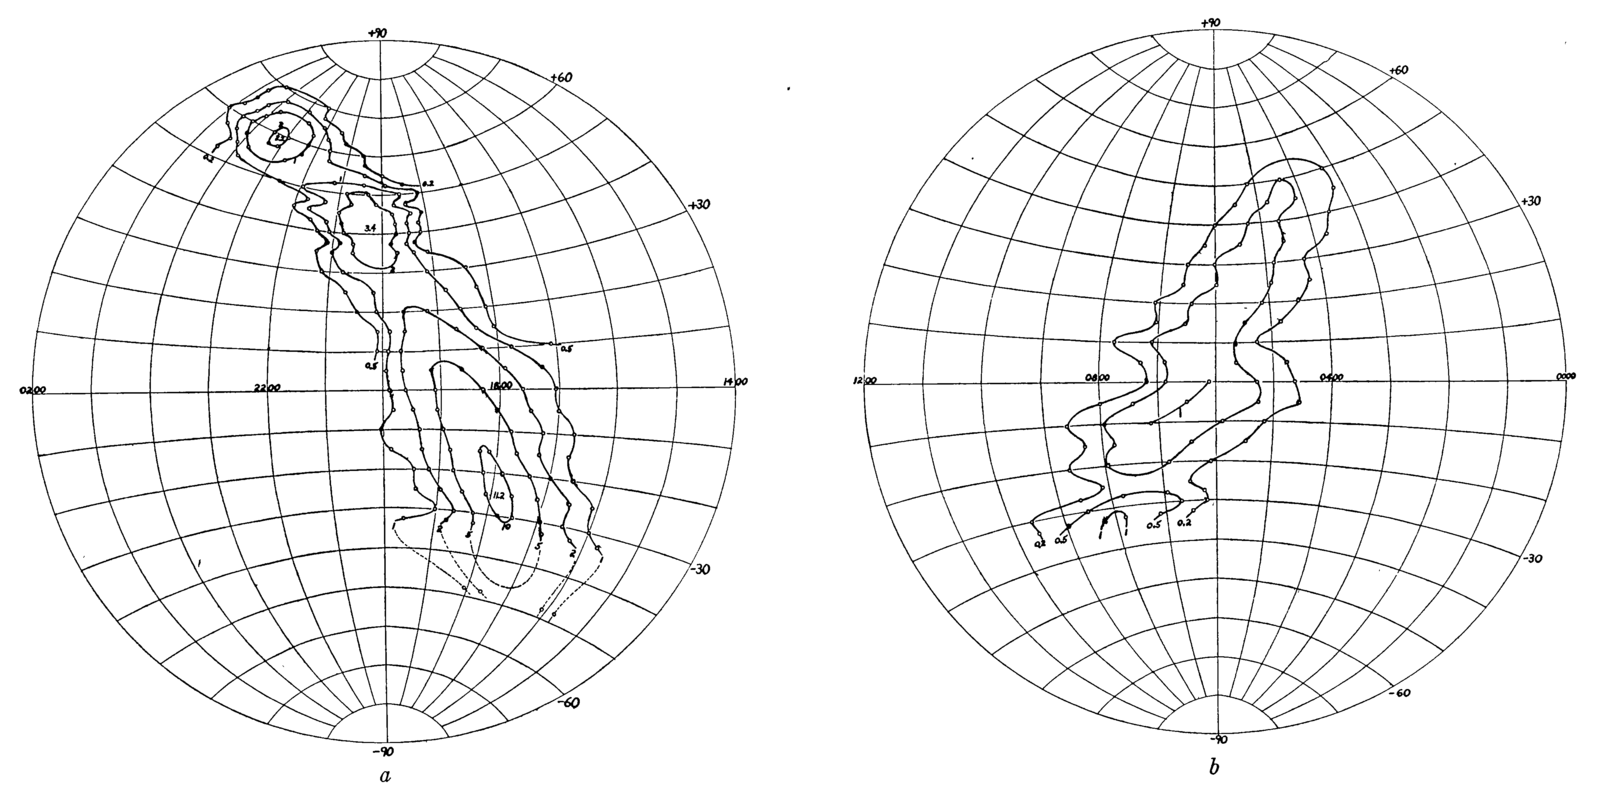
\includegraphics[width=0.8\textwidth]{plots_chp1/Reber_radiomap_1944.png}
     \caption[160 MHz radio map from \citet{Reber1944}]{Intensity contour lines of $\nu_{\rm obs} = 160$ MHz radio emission mapped out by Grote Reber on the self-built 9.5 m paraboloid radio telescope \citep{Reber1944}.}
     \label{fig:Reber-map-sky-1944}
\end{figure}

Both Jansky's discovery and Reber's work were fundamental in introducing the use of radio frequencies in detecting distant objects both within the Milky Way and beyond it. Techniques used in astronomy were developed further through the enhancement of radio receiver technologies used during World War II which led to Baade and Minkowski's own discoveries at the Palomar Observatory, Mount Wilson whose observations showed that two of the sources Reber's first survey detected, Cassiopeia A and Puppis A, spatially coincide with diffuse optical emission referred to as `nebulosities' which were also seen to have large velocity dispersions. Furthermore, the disturbed optical morphology of Cygnus A revealed evidence of it being involved in a galaxy merger \citep{BaadeMinkowski1954}. These cross identifications of a radio sources with optical emission proved that the bright, discrete radio signals picked up by radio surveys were not merely `radio stars' but rather galaxies much like the Milky Way that were emitting powerful bursts of radio emission. Consequently, the term `radio galaxy' was introduced into the astronomy lexicon. 

In order for a radio source to be considered a radio galaxy, an optical counterpart is required due to the fact that redshifts are computed from rest-frame optical, ultraviolet (UV) or near-infrared (near-IR) spectra. Hence, measuring the Doppler shifts of spectral lines at these wavelengths is the primary method for obtaining galaxy redshifts or luminosity distances. Distance is also required to convert the projected sizes of observed components in a galaxy e.g. the extent of the radio lobes (radio sizes) into physical sizes and flux densities into luminosities \citep{Moffet1966}. Once their distances were estimated, radio galaxies became known as the most distant galaxies observable \citep{Stern1999}. 

\section{Motivation}\label{section:motivation}
% M-sigma relation - black-hole and galaxy co-evolution
The empirical $M$-$\sigma$ relation, introduced in section 1.1, states that the mass of the central black-hole ($M_\bullet$) of a galaxy is proportional to its velocity dispersion. This implies that radio galaxies, which generally have high stellar masses, also host very massive central black-holes. They also have high bolometric luminosities ($L_{\rm bol}$) luminosities due to $L_{\rm bol}$ increasing proportionally with the accretion rate as well as the central black-hole mass. 

Based on this, it is rather apparent then that radio galaxies are good places to begin tracing evidence of the kinetic-mode of feedback that occurs within galaxies. There are several other reasons why these particular galaxies are crucial to our understanding of galaxy evolution. 

For one, they provide an opportunity to test theories in cosmology given their detection during redshift epochs that probe the very distant and early Universe at $z\sim4-6$ \citep{LillyLongair1984,Miley1989,Lacy1994a,
Waddington1999,VanBreugel1999,Jarvis2009,Saxena2018}. Their detection up to these high redshifts is essential because by $z\sim6,$ the majority of neutral hydrogen that existed in the Universe during the so-called `Dark Ages' has already been ionised through radiation emitted by the first galaxies and quasars. This early period, referred to as the Epoch of Reionisation (EoR), begins some 150 Myr after the Big Bang (at a redshift of $z\sim11$ and continues up to a cosmic time of 1 Gyr ($z\sim6$) \citep{Zaroubi2013}. Thus, the detection of radio galaxies at high redshifts make them good cosmological probes for parametrising the physics of galaxy formation in the early Universe \citep{Fan2006,Banados2018}.  

% How do galaxies grow / aggregate their mass?
Radio galaxies also allow us to gain better insight into how galaxies aggregate their mass through star-formation in their formative phases. The brightness of stellar emission from galaxies can be determined from optical and near-infrared band magnitudes \citep{GunnOke1975}. In particular, the relation between the brightness of flux measured in the $K$-band (central wavelength: $\lambda_{\rm c}=2.2~\mu$m) which traces redshifted ultraviolet (UV) and optical emission from young stars and redshift show the evolution of flux from stellar emission with cosmic time. This observed relation is known as the Hubble $K$-$z$ diagram (e.g. Fig. \ref{fig:K-z-Lilly1984}). Granted that $K$-band magnitudes are detectable at redshifts of up to $z<4,$ the empirical $K$-$z$ relation for ensembles of radio sources can be used to test cosmology and galaxy evolution models  \citep{LillyLongair1984,EalesRawlings1996,Eales1997}. More recently, the work of \citet{Inskip2002} showed that the $K$-$z$ relation for a sample of radio galaxies fits reasonably to an Einstein-de Sitter cosmology model for a matter density ($\Omega_{\rm M}$) and dark energy density ($\Omega_\Lambda$) of ($\Omega_{\rm M}=1, \Omega_\Lambda=0$). Despite $\Omega_\Lambda=0$ being ruled out by better constraints of cosmological parameters by \citet{Planck2016} measurements from the cosmic microwave background (CMB), these studies still display the potential usefulness of the $K$-$z$ diagram to cosmology.  

\begin{figure}[!ht]
    \centering
    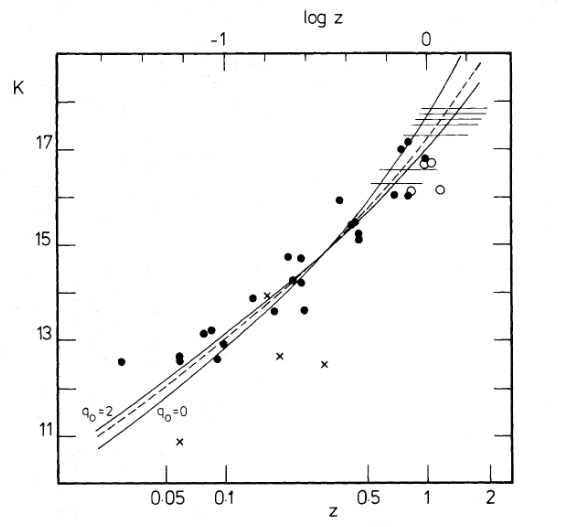
\includegraphics[width=0.8\textwidth]{plots_chp1/K_z_Lill1982.png}
    \caption[Near-infrared Hubble $K$-$z$ diagram \citep{LillyLongair1982}]{Infrared Hubble $K$-$z$ relation from \citet{LillyLongair1982} and is shown for cosmological deceleration parameters $q_0=0$ and $q_0=2$ against the observed magnitudes.}
    \label{fig:K-z-Lilly1984}
\end{figure}

% fix this paragraph ....
The $K$-$z$ diagram has become a widely used diagnostic for placing constraints on galaxy evolution models given its low level of scatter. The work of \citet{rocca-volmerange2004} makes use of the $K$-$z$ diagram to predict the stellar masses of radio galaxies, in this work. Results indicate that the apparent (observed) $K$-band of the ensemble of radio galaxies originally compiled by \citet{debreuck2002a} and first detected in the Third and Sixth Cambridge Catalogues of Radio Sources (3CR and 6CE) discussed later in section \ref{section:early-radio-surveys}. The galaxies are detected over the redshift range $0 \leq z \leq 4$ and shown against galaxy evolution models which predict the baryon masses of elliptical galaxies (see Fig. \ref{fig:K-z-rocca-volmerange2004-pegase}). For the radio galaxies, the results show that their baryon masses ($M_{\rm bary}$) lie within the range, $10^{11} < M_{\rm bary}/\rm{M}_\odot < 10^{11.5}$ and have an upper limit of $M_{\rm bary}/\rm{M}_\odot < 10^{12}$ imposed on all galaxy types. 

\begin{figure}[!ht]
  \centering
  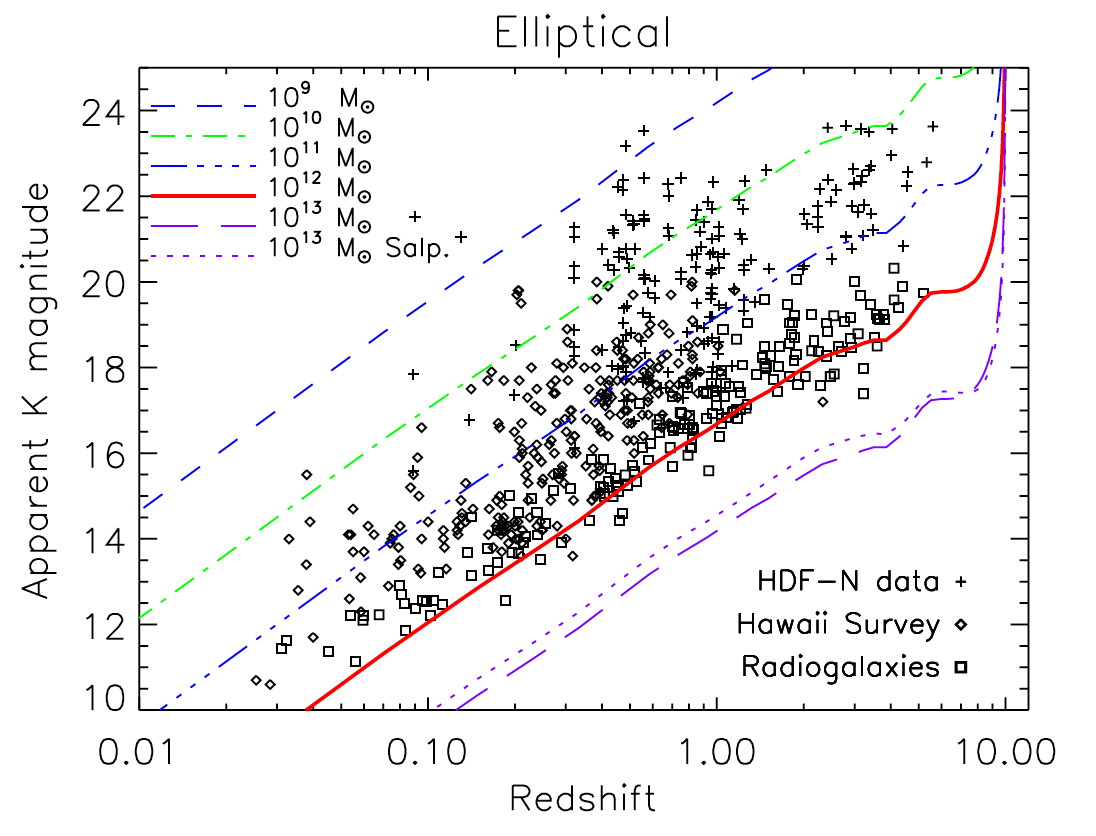
\includegraphics[width=0.8\textwidth]{plots_chp1/K_z_Rocca-Volmerange_2004_pegase.png}
  \caption[$K$-$z$ diagram for elliptical radio galaxies from \citet{rocca-volmerange2004}]{The $K$-$z$ diagrams of radio galaxies (squares) from 3CR and 6CE. The data also includes $K$-band magnitudes of field galaxies from the Hawaii Survey \citep{Songaila1994} (diamonds) and HDF-N \citep[Hubble Deep Field-North;][]{Dickinson2003} (crosses). The initial mass function (IMF) models from \citet{RanaBasu1992} which are given for a range of baryon masses from $M_{\rm bary} = 10^9 - 10^{13}$ M$_\odot.$ A top-heavy (TH) IMF model for $M_{\rm bary} = 10^{13}$ M$_\odot$ is included for comparison.}
  \label{fig:K-z-rocca-volmerange2004-pegase}
\end{figure}

The predicted range of radio galaxy baryon masses from \citet{rocca-volmerange2004} are in agreement with those obtained by \citet{seymour2007} who make use of data from the {\it Spitzer Space Telescope} (SST) \citep{Werner2004}. Datasets comprising SST near-IR photometry for 69 radio galaxies between redshifts of $1.0 < z < 5.2.$ The {\it Spitzer} photometry obtained by the instruments on board the telescope namely the Infrared Array Camera (IRAC; $3.6-8.0~\mu$m), Infrared Spectrograph (IRS; 16 $\mu$m) and Multi-band Imaging Photometer (MIPS; $24-160~\mu$m). Spectral energy distribution (SED) models that aimed to disentangle the stellar, dust and AGN components within the optical and near-IR emission were fit to the IR data. The stellar masses were obtained from $H$-band magnitudes (at a central wavelength of $\lambda_{\rm c} = 1.65$ $\mu$m)\footnote{The choice to use $H$- rather than $K$-band magnitudes is motivated by galaxy evolution models which show that the predicted flux of radio galaxies peaks at the central wavelength of the $H-$band. Additionally, SED-fitting in \citet{Drouart2012} showed that the $H-$band is optimal for sampling the stellar mass without the SED being too contaminated by emission from heated dust.}. The result of this study shows that the radio galaxies have stellar masses (M$_*$) within the range of $10^{11} < M_* < 10^{11.5}$ M$_\odot.$  Radio galaxies, therefore, give us insight into what drives the formation and evolution of galaxies at the high stellar mass end.

% How are jets formed?
Observations of radio galaxies provide us an incredible wealth of information concerning the physical processes that occur within radio galaxies. Although they provide a real-world view of astrophysical objects as they existed, with the caveat of observational biases included, they only provide snapshots of the object at a given epoch. A simulation, although controlled by man instead of nature, provides us with a continuous and evolving view of a galaxy. Hydrodynamical simulations have provided a simulated view of radio jets and the impact they bear on the surrounding gas medium through which they propagate. This has been done by \citet{krause2002} and \citet{krause2005} who demonstrate that shells of neutral hydrogen gas are responsible for absorption troughs observed in hydrogen Lyman-alpha line (\ion{H}{i} Ly$\alpha$) at $1215.67~\text{\AA}$ in the spectra of high redshift radio galaxies (HzRGs). The neutral hydrogen (\ion{H}{i}) gas shells that scatter and absorb Ly$\alpha$ photons can form at the bow shock fronts of radio jets through shock-driven compression of gas. Given sufficient time (over Gyr time-scales), \ion{H}{i} gas shells disintegrate at the shock front of the jets as a result of Rayleigh-Taylor instabilities in the gas medium. 

Another example of simulations which demonstrate the effect of jets on ISM gas are those of \citet{Gaibler2011}. These Monte Carlo 3D simulations depict the propagation of radio jets into a clumpy interstellar medium (ISM). The passage of the radio jets and their impact on the surrounding ISM is shown in time snapshots that illustrate the impact of radio jets on the surrounding gas medium at three different moments during the duty cycle of the radio jet (see Fig. \ref{fig:jet-ism-Gaibler2011}). 

The average duty cycle of radio jet activity persists over a time-scale of $\tau_{\rm jet} \simeq 10 - 100$ Myr. Simulations of jet-gas interactions indeed suggest that radio galaxies are prime targets to study when seeking to understand the impact that radio jets have on ISM gas that lies in proximity to the AGN in radio galaxies.

\begin{figure}[!ht]
  \centering
  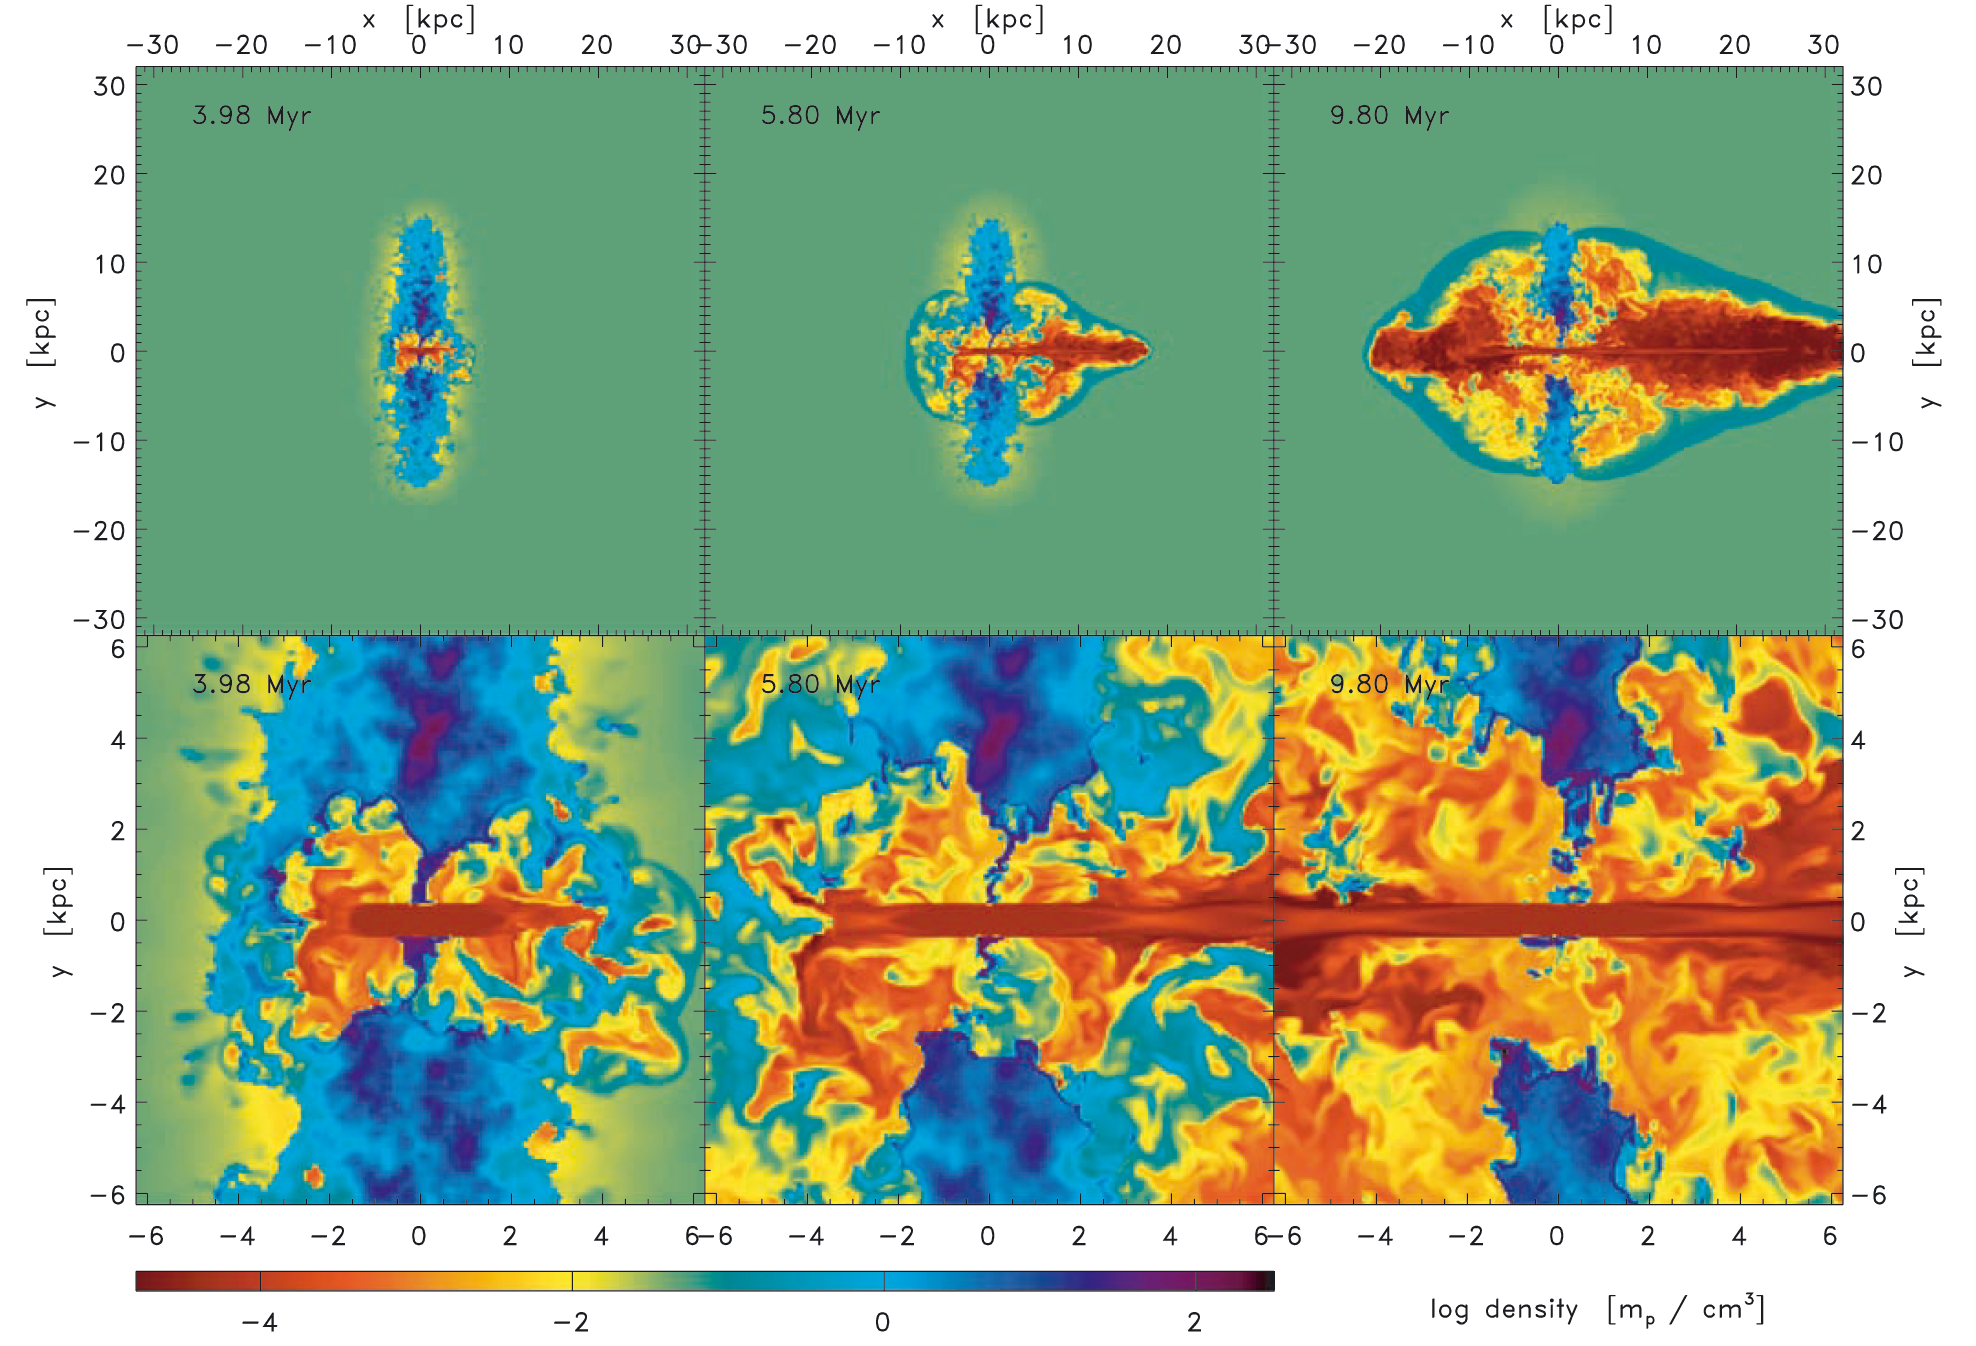
\includegraphics[width=\textwidth]{plots_chp1/jet_gas_sims_Gaibler_2011.png}
  \caption[Simulation snapshots of bi-conical radio jet from \citet{Gaibler2011}]{Snaphots of 3D Monte Carlo simulations of a bi-conical radio jet pummelling through a disc-shaped clumpy interstellar medium with log-normal density distribution in \citet{Gaibler2011}. The growing radio jet begins to plough through the clumpy ISM medium at $t=3.98$ Myr. At $t=5.80$ Myr, an asymmetry in the lobes formed by the relativistic jets has already formed. After $t=9.8$ Myr has passed (the average duty cycle of a radio AGN), extended asymmetric radio lobes enclosed in a bow-shock region are apparent. The upper panel shows a large-scale view of the simulation with the lower panel providing a closer view of the core activity.}
  \label{fig:jet-ism-Gaibler2011}
\end{figure}

%% How could kinetic-mode of feedback affect SF ? 
Radio galaxies at high redshifts are known to form stars rapidly with star-formation rates (SFR) of $\rm SFR \gtrsim 100 - 1000$ M$_\odot \rm yr^{-1}$ inferred from SED fitting to near-IR photometry \citep{Drouart2014,falkendal2019}. The resulting SFR and black-hole accretion rates inferred from the SED-fitting are plotted in Figs \ref{fig:SFR_AGN_LIR-Drouart} and \ref{fig:SFR_AGN_LIR-Falkendal}. Additionally, the Main Sequence of star-forming galaxies which defines the expected SFR for a galaxy of given stellar-mass, is included in the discussion in order to determine how ``normal'' HzRGs are. This normalcy is quantified by the galaxy's shift in relation to the Main Sequence i.e. $\Delta$(M.S.). 

This comparison has been done by \citet{falkendal2019} whose HzRGs sample is shown against the Main Sequences of star-forming galaxies in Fig. \ref{fig:HzRGs-MS-Falkendal2019}. What is clear from these plots, is that at $z > 3,$ more of the HzRGs have slightly lower SFR than is expected for their stellar masses. This implies that, although HzRGs form stars rapidly, they appear to be in a process of quenching. At later epochs, $ 1.3 < z < 3,$ the HzRGs have SFR and $M_*$ that are more consistent with the Main Sequence. Therefore, HzRGs are likely to have undergone earlier phases of rapid star-formation that has begun to slow down by $z\sim3.$ This may be due to AGN jet feedback driving outflows of molecular gas that fuels star-formation.

\begin{figure}[!ht]
    \centering
    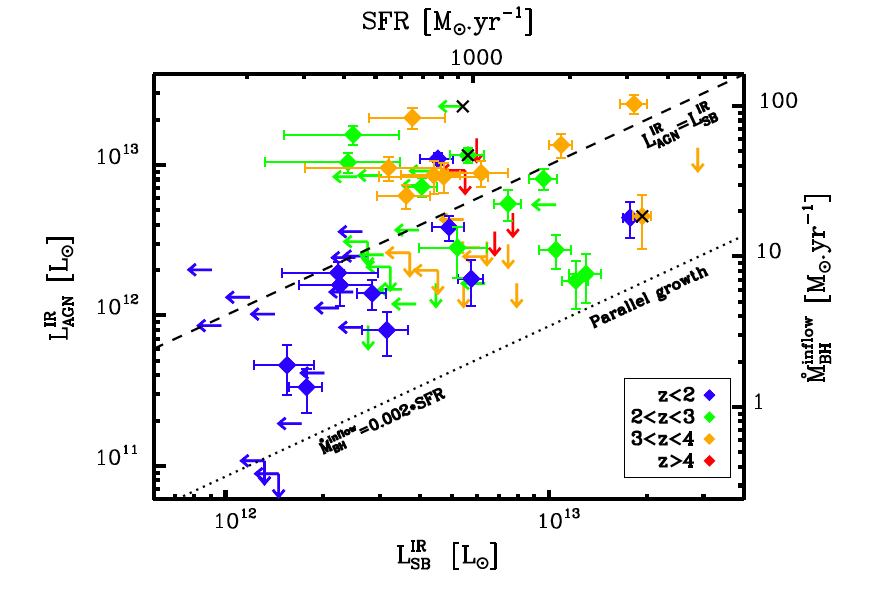
\includegraphics[width=0.95\textwidth]{plots_chp1/SFR_AGN_LIR_Drouart_2014.png}
     \caption[AGN vs SF luminosity from \citet{Drouart2014}]{The total AGN luminosity, $L^{\rm IR}_{\rm AGN}$ as a function of the star-forming luminosity $L^{\rm IR}_{\rm SF}$ from \citet{Drouart2014}. The top axis converts $L^{\rm IR}_{\rm SB}$ to SFR using the \citet{Kennicutt1998} relation. The right axis converts $L^{\rm IR}_{\rm AGN}$ to $\dot{M}_{\rm BH}$ assuming $\epsilon=0.1$ and $\kappa^{\rm Bol}_{\rm AGN}.$ The dashed line marks $L^{\rm IR}_{\rm AGN} = L^{\rm IR}_{\rm SB}.$ This dashed line indicates the relation corresponding to $\dot{M}_{\rm BH} = 0.024 \times \rm SFR,$ using the right and top axes. The dotted line represents the parallel growth mode, where black holes and galaxies grow simultaneously, following the $M_{\rm BH}$-$M_{\rm Gal}$ relation.}
     \label{fig:SFR_AGN_LIR-Drouart}
\end{figure}     
    
\begin{figure}[!ht]
	\centering
    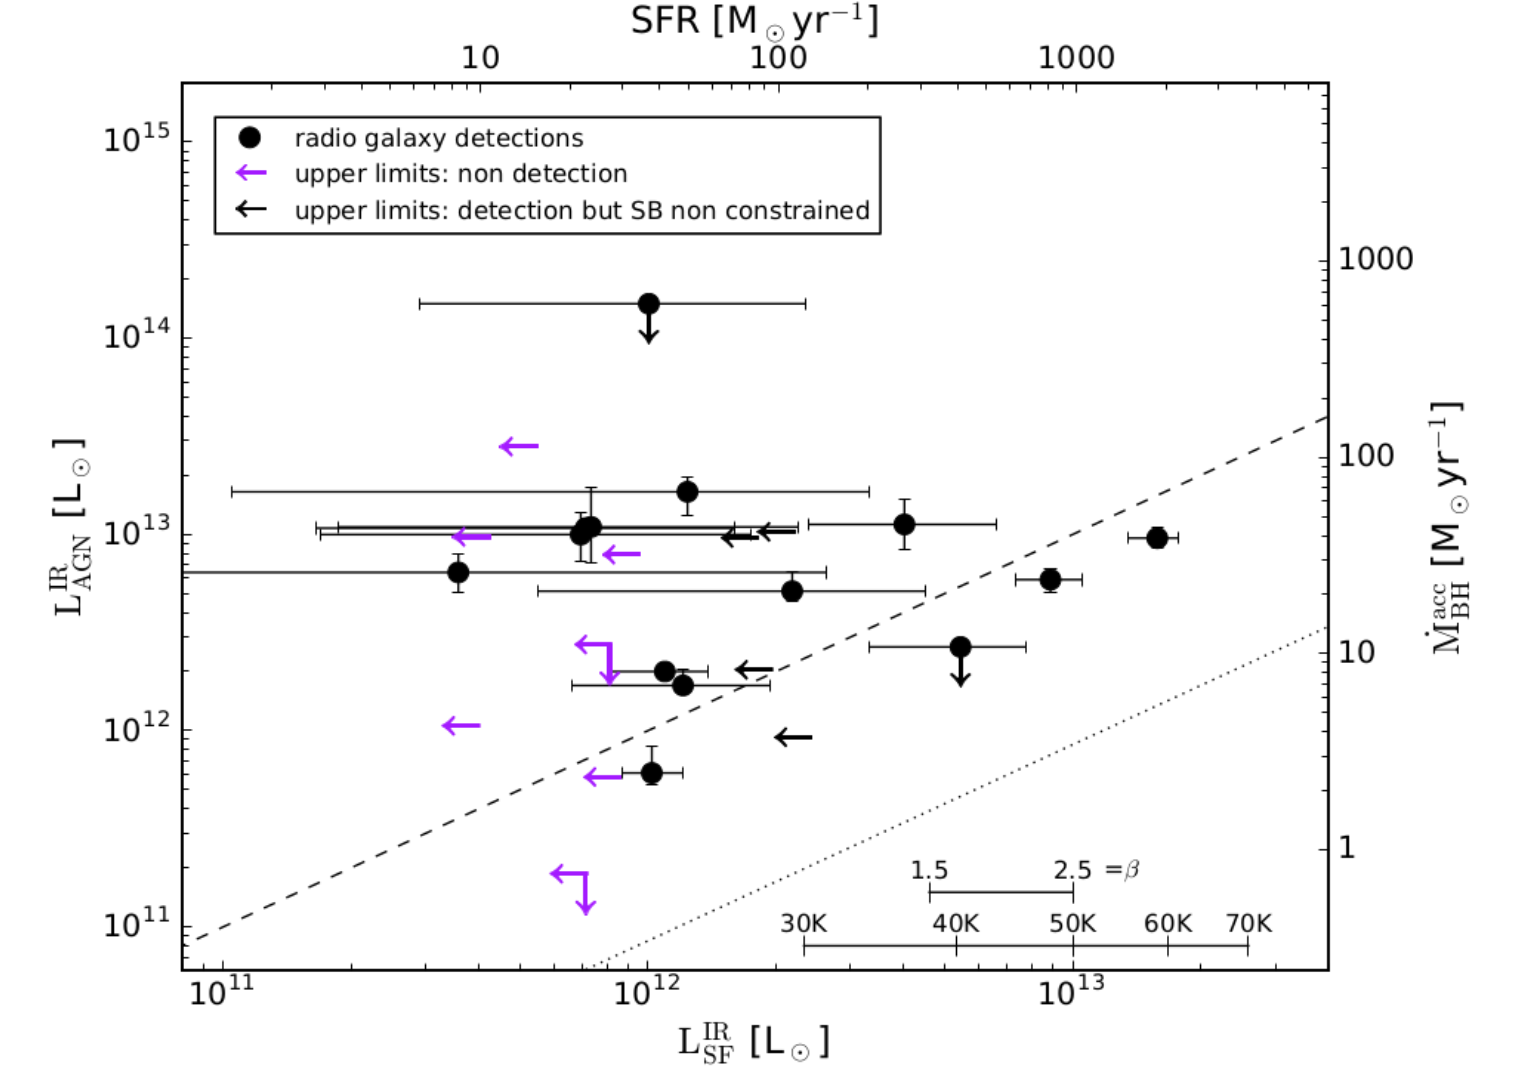
\includegraphics[width=0.8\textwidth]{plots_chp1/SFR_AGN_LIR_Falkendal_2019.png}
    \caption[AGN vs SF luminosity from \citet{falkendal2019}]{$L^{\rm IR}_{\rm AGN}$ as a function of $L^{\rm IR}_{\rm SF}$ from \citet{falkendal2019}. The dashed black line represents equality between the ordinate and abscissa which also represent the star-formation rate (SFR) and black-hole (BH) mass accretion rate ($\dot{M}^{\rm acc}_{\rm BH}$). The dotted shows the axis where black-hole accretion rate $\dot{M}^{\rm acc}_{\rm BH} = 0.002 \times \rm SFR$ which demarcates parallel growth mode where the galaxy and black hole grow in tandem and obey the spheroid mass-BH mass relation.}
    \label{fig:SFR_AGN_LIR-Falkendal}
\end{figure}

\begin{figure}[!ht]
   \centering
   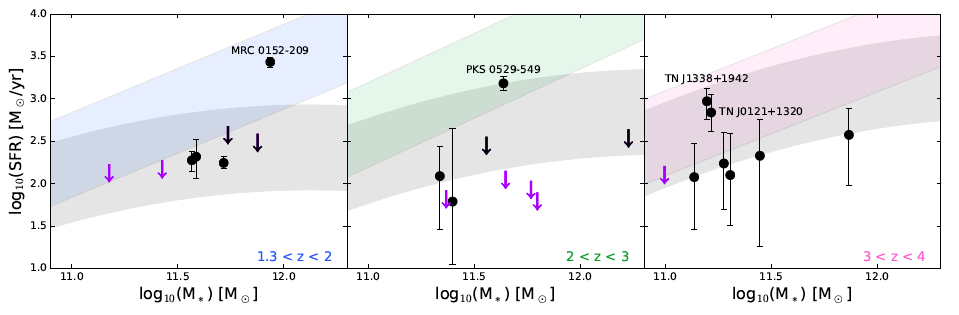
\includegraphics[width=\textwidth]{plots_chp1/HzRGs_main_sequence_Falkendal2019.png}
   \caption[HzRGs relative to Main Sequence in \citet{falkendal2019}]{HzRGs from \citet{falkendal2019} sample are compared to the Main Sequences in the grey shaded regions are taken from \citet{Schreiber2015} while the Main Sequences in colour are those from \citet{Santini2017}.}
   \label{fig:HzRGs-MS-Falkendal2019}
\end{figure}

The Lilly-Madau plot of cosmic star-formation rate density (SFRD) is well known in astronomy and presents an intriguing puzzle that astronomers continue to work on solving \citep{Lilly1995,Madau1996}. The plot shows that at $z \simeq 1.9$ (3.5 Gyr after the Big Bang) the level of cosmic star-formation per epoch per volume reaches a peak as Fig. \ref{fig:SFRD_z_Madau_Dickinson2014} illustrates \citep{MadauDickinson2014}. It is now known that only populations of galaxies that follow the Main Sequence relation can have a significant effect on the cosmic SFRD at $1 < z < 3$ therefore HzRGs, which are found on the main sequence at these redshifts, may be important in explaining why the function, $\psi(z),$ takes on this shape. Unlike normal main-sequence star-forming galaxies which follow the M.S., radio galaxies host powerful jets that have a unique impact on the gas that is gravitationally bound to a galaxy and in close proximity to the AGN. Hence, they hold great importance in providing clues on how star-formation is affected by jet-driven gas outflows. 

\begin{figure}[!ht]
   \centering
   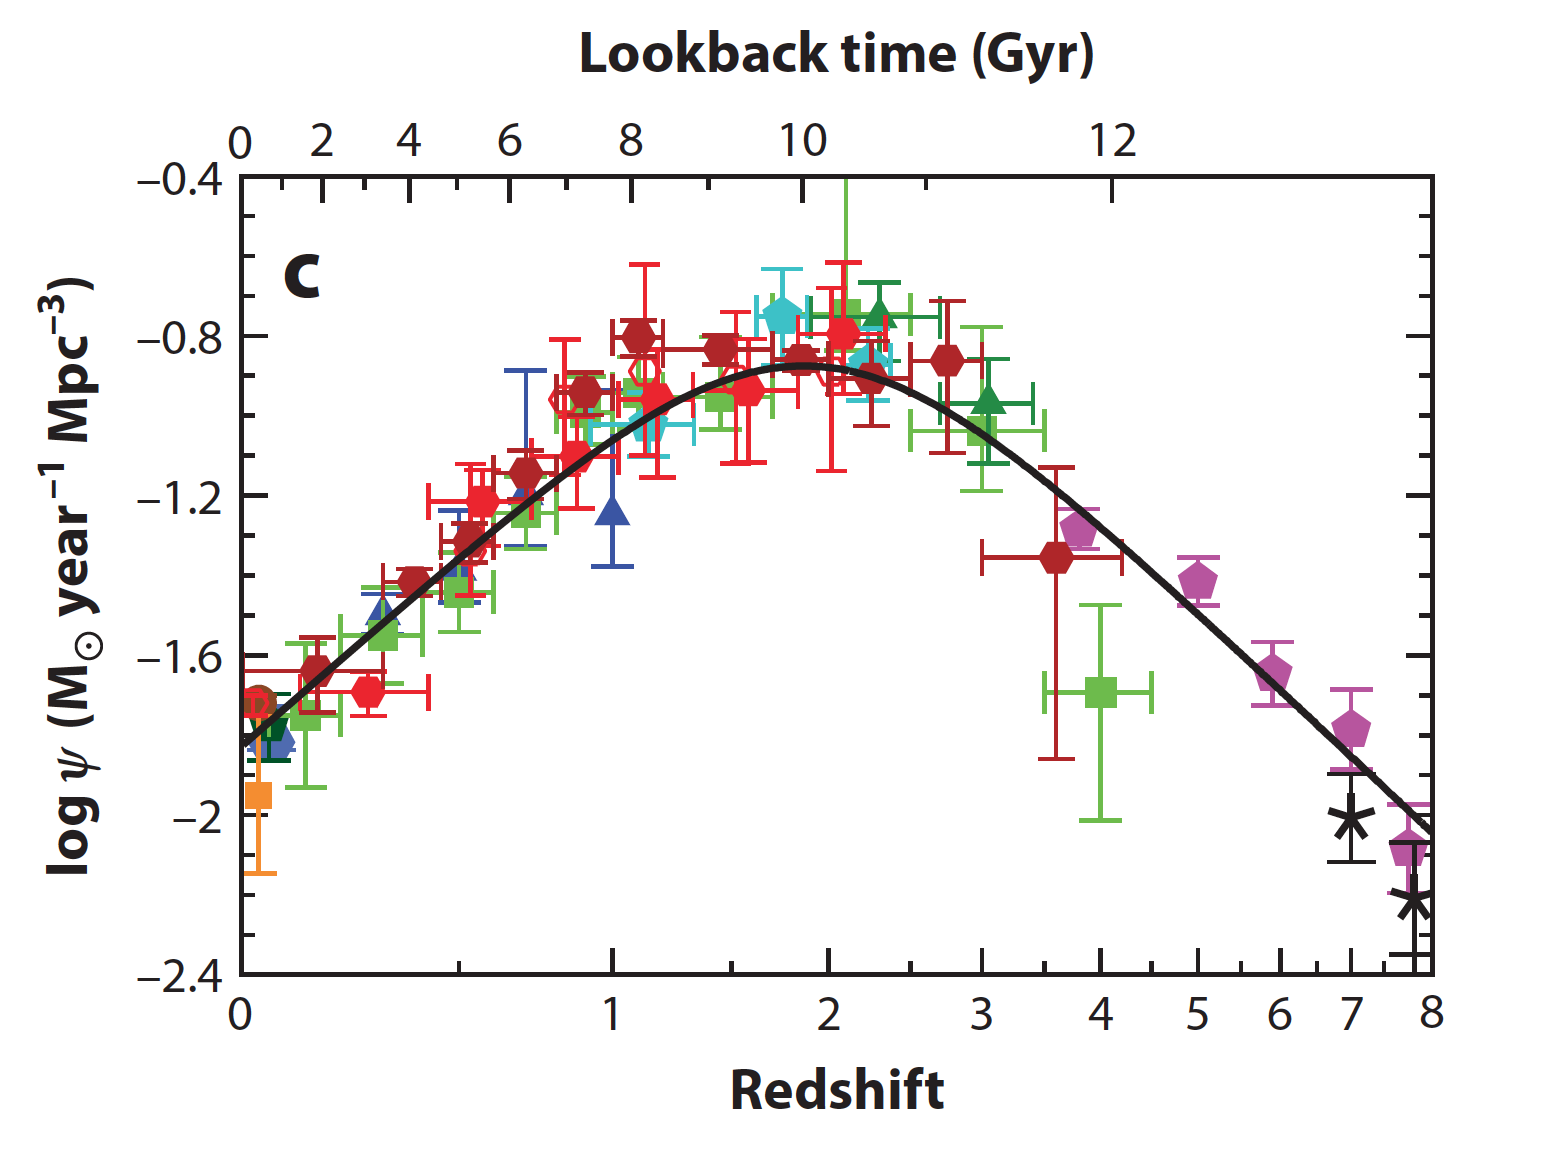
\includegraphics[width=0.8\textwidth]{plots_chp1/SFRD_z_Madau_Dickinson_2014.png}
   \caption[SFRD as a function of redshift in \citet{MadauDickinson2014}]{The star-formation rate density (SFRD) or $\psi(z)$ in M$_\odot$ yr$^{-1}$ Mpc$^{-3}$ given as a function of redshift as well as look-back time in Gyr. The measurements shown are obtained from far ultraviolet (FUV) and near-infrared (NIR) rest-frame luminosities which have been converted to SFR. In the FUV, the equation SFR $= \kappa_{\rm{FUV}} \times L_\nu (\rm{FUV})$ while in the NIR, it is obtained via SFR $= \kappa_{\rm{IR}} \times L_{\rm{IR}}.$}
   \label{fig:SFRD_z_Madau_Dickinson2014}
\end{figure}

\section{Radio Galaxies} 
\subsection{Early radio surveys}
In the wake of Jansky's discovery of cosmic noise, Reber's 160 MHz radio survey and Baade and Minkowsi's identification of radio galaxies, a number of radio surveys were successfully completed. Studies carried out using these surveys' data have resulted in an increase in the number of known radio radio galaxies. 

The Third Cambridge Catalogue \citep[3C;][]{Edge1959} was assembled using the Cambridge Interferometer and is one of first and most prolific radio survey catalogues known. The first and second Cambridge catalogues (1C and 2C) were also compiled in Cambridge during 1950 \citep{Ryle1950} and 1955 \citep{Shakeshaft1955}. Despite being the first Cambridge radio survey catalogues, however, 1C and 2C source detections were affected by astronomical `confusion' - a consequence of more than one astronomical source being detected within one synthesised beam aperture. The result being that several sources are incorrectly resolved as one source. Hence, 3C, which managed to overcome this problem is perhaps the first and most reliable of the Cambridge catalogues to identify a significant number of radio galaxies including 3C 295 which was the most distant radio galaxy known at the time of its discovery \citep{Minkowski1960}. 

The revised 3C Catalogue \citep[3CR;][]{Leslie1961,Bennett1962} observed at $\nu_{\rm obs} = 178$ MHz at a sensitivity or flux limit of $S_{178} = 9$ Jy contained a large number of bright sources at declinations, $\delta > -5^{\circ}$ - in the northern hemisphere. A radio interferometer at the Palomar Observatory Sky Survey \citep[POSS;][]{Veron1966} identified optical counterparts to a number of 3C sources to accurately calibrate the radio source positions and determine whether the optical and radio detections coincide spatially or are related to the same source. More revision of the original 3C source list was carried out by \citet{LaingRileyLongair1983} forming the 3CRR catalogue ($S_{178} \geq 10$ Jy) which contained sources that had yet to be detected due to the flux limitations of the original 3C survey. 

Some of the more notable catalogues that followed were 4C \citep{PilkingtonScott1965} observed at a frequency of $\nu_{\rm obs} = 178$ MHz and a flux limit of $S_{178} = 2$ Jy. This catalogue was crucial in identifying sources that have radio spectral indices ($\alpha$) of $\alpha < -1$ in the flux density-frequency relation $S_\nu \propto \nu^{\alpha}.$ Selecting sources with $\alpha < -1$ led to the identification of sources with small angular sizes and high radio luminosities suggesting that the sources were at significantly greater distances than those with less steep spectra or $\alpha > -1$ \citep{Tielens1979}. The steep spectrum radio sources were added to the 4C Ultra Steep Spectrum Sample \citep[4C/USS;][]{ChambersMiley1990} which consisted of furthest radio galaxies known at the time: 35 of which are at $z > 2$ and 2 at $z > 3.$ The legacy of Cambridge catalogues has continued on through the years leading up to the most recent 10C Survey  \citep{AMIConsortium2011}. 

Another notable radio survey is the Molonglo Reference Catalogue of Radio \citep[MRC;][]{Large1981} which comprises 12,141 sources detected at a tuning frequency of $\nu_{\rm obs} = 408$ MHz at a flux limit of $S_{408} \geq 0.7$ Jy on the Molongolo Radio Telescope \citep{Hunstead1972}. From MRC, steep spectrum sources with $\alpha < -0.9$ were selected at $S_{408} >0.9$ Jy. The steep spectrum sources in this catalogue also have accompanying optical long-slit spectroscopy which identified the majority of the galaxies as having redshifts of $z > 0.8$ \citep{McCarthy1990}. On a subset of the MRC sources with flux densities, $S_{408} >0.95$ Jy and redshifts, $z > 1$ radio galaxies were observed to have extended filaments of optical emission and higher luminosity radio cores and jets than galaxies from the 3C catalogue \citep{McCarthy1991}. 

Many efforts made to build up source catalogues from radio interferometric surveys during the early days of radio astronomy have provided an extensive repository of radio galaxies. This means that we now have a sufficiently wide database from which to study the evolution of radio galaxies from their early formation after the Epoch of Reionisation all the way to the present-day epoch where we observe galaxies in the nearby Universe. 

\subsection{Radio galaxies across cosmic time}
As the large-scale structure of the Universe changes with time as a result of cosmic expansion \citep{Planck2016}, so do the physical properties of galaxies. One of the main goals of this thesis, in fact, is to compare and contrast the properties of radio-loud AGN host galaxies at high and low redshift. In this section, I highlight some the known commonalities and disparities of these galaxies at the different redshift epochs where they are found.  

Radio galaxies are empirically defined as radio-loud sources that have double-lobed morphologies formed through the expulsion of synchrotron radiation from bipolar (bi-directional) jets emitted from their cores. A perfect illustration of this is the nearby galaxy Cygnus A ($z=0.057$), a local radio galaxy first identified by \citet{JennisonDasGupta1953}. Early and more recent interferometric observations shown in Fig. \ref{fig:CygA} exhibit quite nicely its double-lobed radio structure \citep{Moffet1966,CarilliBarthel1996}. Thus, provided that a radio galaxy is at a sufficiently low-redshift for its radio structure to be resolved, its double radio morphology will be apparent. An important cosmological effect makes these morphologies apparent at large distances. It just so happens that at $z > 1,$ the angular diameter distance drops down gradually rather than steeply while the cosmic brightness decreases by a factor of $(1+z)^{-4}.$ This means that the physical sizes of radio lobes do not vary greatly with increasing redshift at $z > 1.$ From radio observations, we know that high-redshift radio galaxies have double-lobe structures that can extend out to $\sim$100 kpc in size and can be resolved even up to $z \lesssim 4$ \citep{Miley1980,carilli1997,pentericci1999}.  

The double-lobe morphologies place them in the category of Fanaroff-Riley II sources which have extended lobes that terminate at edge-brightened hotspots where non-thermal radiation increases in surface-brightness \citep{FanaroffRiley1974}. Their double-lobe morphology also implies that the relativistic jets are oriented along the plane of the sky. Indeed, the orientation of the jets are an important means by which radio sources are classified. A Type 1 radio AGN or quasar has `beamed' jets where the observer looks into the barrel of the ionisation cone. On the other hand, the Type 2 AGN refers to sources with jets that are observed parallel to (or at a small angle from) the plane of the sky. Therefore, by definition, all radio galaxies are Type 2 AGNs. 

Radio galaxies have classically been dichotomised into radio-loud and quiet populations based on their observed radio luminosities. This bi-modality was initially identified in quasar populations. Since radio galaxies are likely to have hidden or dust-obscured quasars at their nuclei, the bi-modal description can be extended to them as well \citep{vernet2001}. 

Generally, radio-loud sources, which are rarer than radio-quiet ones, have comparatively higher radio luminosities and are hosted by elliptical galaxies \citep{Padovani1993} while radio-quiet sources are not \citep{Wilson1995}. Also, the lower limit for radio-loud sources is defined by radio luminosities of $L_{1.4~\rm GHz} \gtrsim 10^{25}$ W Hz$^{-1}$ or $L_{5~\rm GHz} \gtrsim 10^{26}$ W Hz$^{-1}$ \citep{Miller1990}. More recently, radio luminosity functions of sources in the local Universe have shown that the star-forming galaxy populations that do not form jets outnumber AGN by a factors of up to 10 at $L_{1.4~\rm GHz} \lesssim 10^{23}$ W Hz$^{-1}.$ Thus, even though star-forming galaxies may be detectable at radio frequencies, their luminosities tend to be significantly lower than those of radio-loud AGN \citep{Best2005a}. 

The widely accepted theory of jet-formation states that radio jets are formed through synchrotron radiation which is emitted as a result of the acceleration of electrons by magnetic fields. The free electrons are sourced from a plasma surrounding the central black-hole where neutral gas is sufficiently heated and ionised by radiation emitted by the AGN. This so-called synchrotron radiation theory was first proposed by \citet{Shklovskii1953} who stated that synchrotron radiation can power relativistic jets which, over Myr time-scales, form the extended radio lobes with sizes in the order of $\sim$100 kpc. Given that the sources are radio-loud with luminosities detected in radio frequencies of $L > 10^{25}$ W Hz$^{-1}$ and the average lifetime of a radio source (its duty cycle) falls within a range of $\tau \simeq 10-100$ Myr, synchrotron radiation is sufficient to fill radio lobes with energies of up to $E \simeq 10^{60}$ erg assuming an AGN duty cycle of $\tau = 100$ Myr and $L_{\rm AGN} = 10^{46}$ erg. How the radio jets are launched, however, is still largely up for debate.

\begin{figure*}[!ht]
  \centering
  \subfloat[The nearby ($d_{\rm L} = 256.3$ Mpc) radio galaxy, Cygnus A, observed with the Cambridge Telescope with a synthesised beam of $23'' \times 35''$ observed at $\lambda=21$ cm. The corresponding radio contours show the double-lobed morphology. The radio contours are superimposed over an optical image taken using the Hale Reflector Telescope. The optical image has a $4' \times 6'$ wide field-of-view \citep{Moffet1966}.]{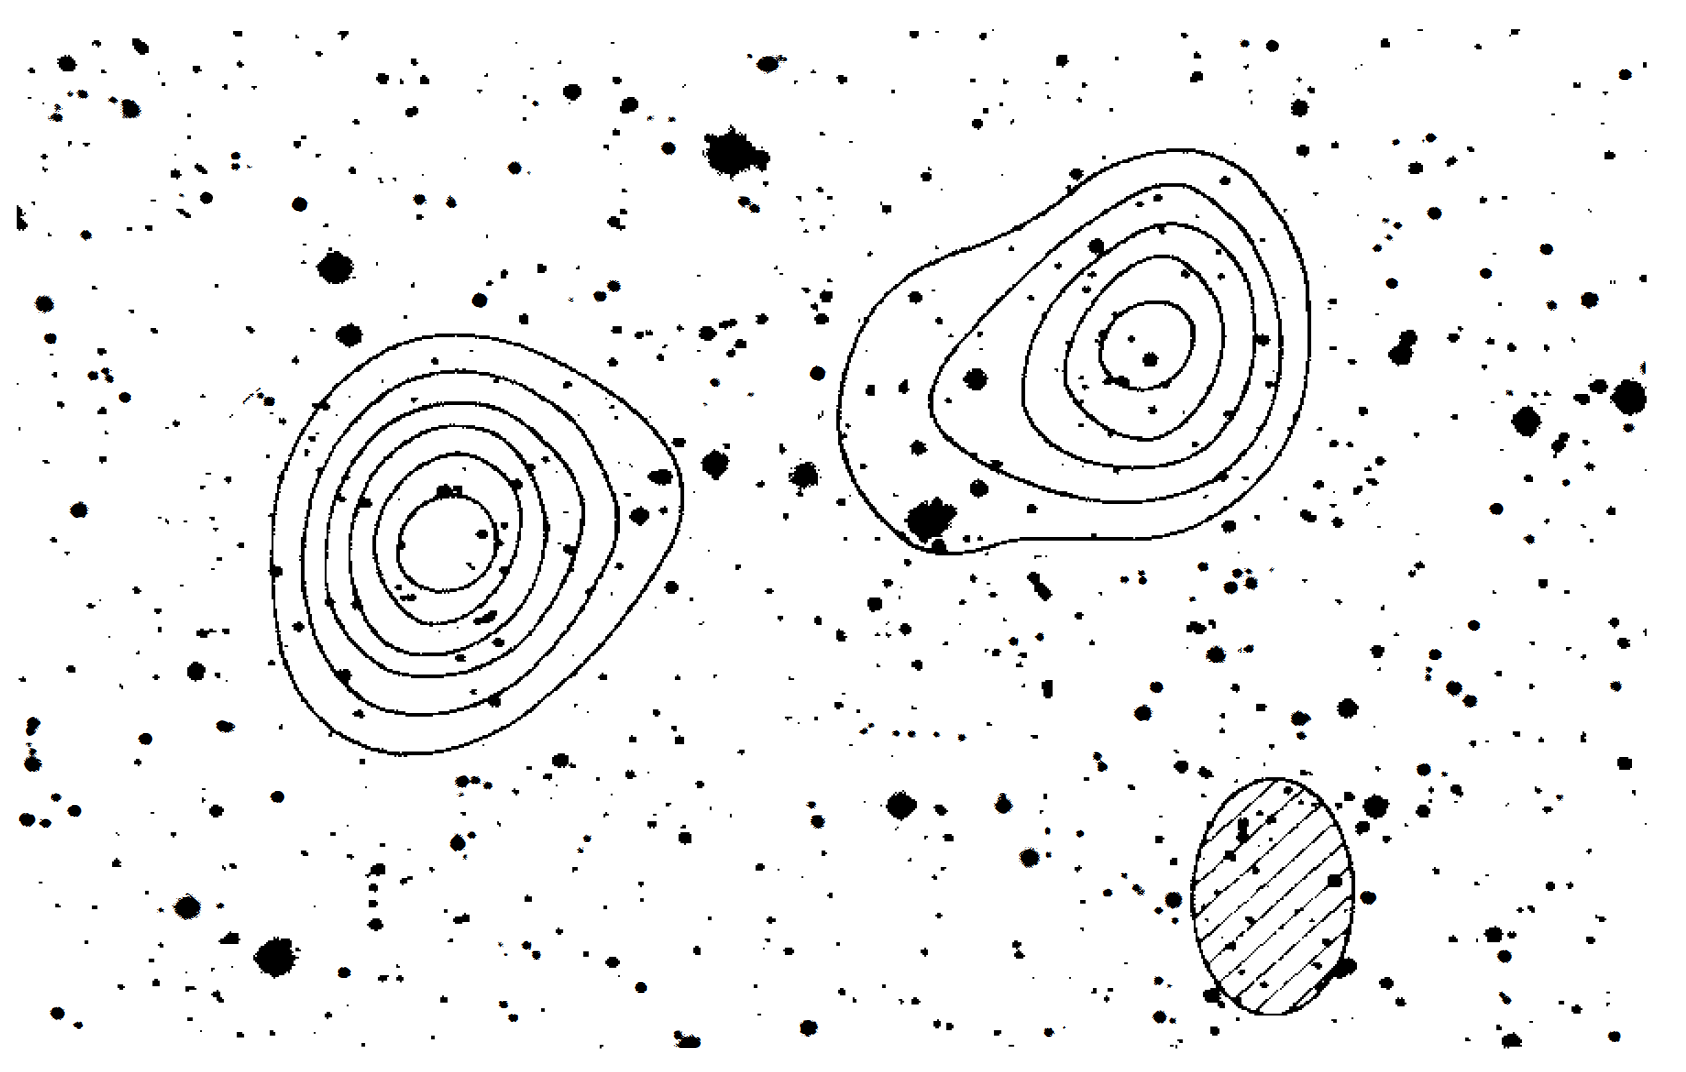
\includegraphics[width=0.9\textwidth]{plots_chp1/Cygnus_A_Hale_Baade_1965.png}}\\
  \subfloat[Cygnus A observed with the Very Large Array (VLA) at tuning frequency of $\nu_{\rm obs} = 5$ GHz \citep{CarilliBarthel1996}.]{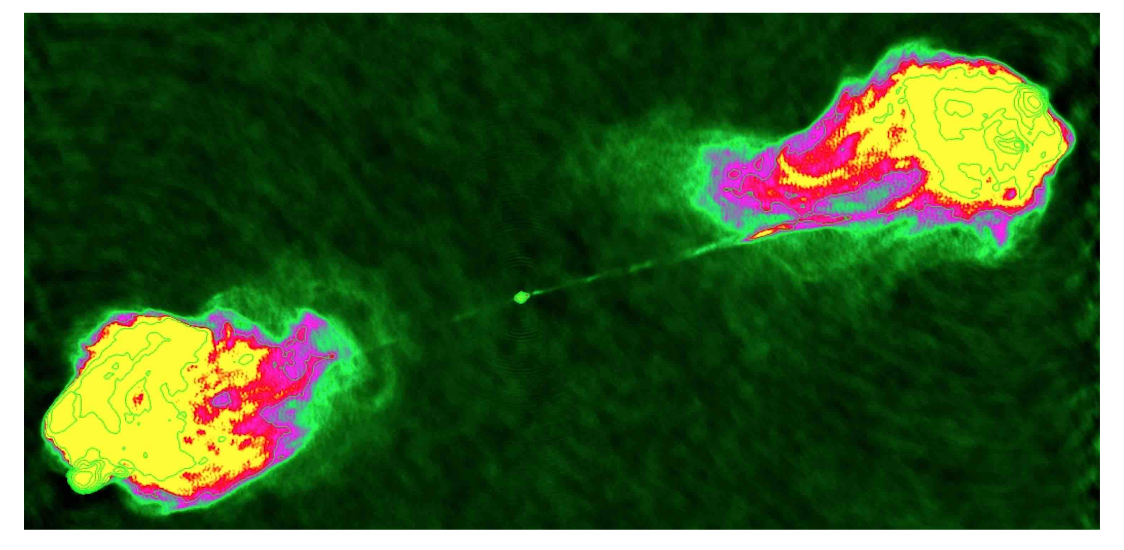
\includegraphics[width=0.9\textwidth]{plots_chp1/CygA_Carilli_Perley.png}}
  \caption[Cygnus A radio imaging in 1966 and 1996]{Radio images of Cygnus A in 1966 and 1996.}
  \label{fig:CygA}
\end{figure*}

The existence of galactic scale magnetic fields is confirmed, furthermore, through the polarisation of light emitted from the AGN. With many observations of polarized emission in radio galaxies having already been carried out by synchrotron radiation has increasingly become a more plausible explanation for the cause of radio jet emission. Radio polarisation studies also show that radio polarisation generally increases with redshift. The degree of polarisation is quantified by the rotation measure (R.M.) defined as,

\begin{equation} 
R.M. = \frac{e^3}{2\pi m_e^2 c^4} \int_0^L n_e(l)B_{||}(l)dl.
\end{equation}

The rotation measure is observed to be stronger at high-redshift than in radio galaxies at $z < 1$  \citep{Saikia1988,Scarrott1990,Tadhunter1992,Jannuzi1991,diSeregoAlighieri1993,
Tran1995,Jannuzi1995,diSeregoAlighieri1996,Jones1996,Feretti1999,Taylor2002,Kaczmarek2018}.
In section \ref{section:early-radio-surveys}, the ultra steep spectrum bias for selecting distant radio galaxies was introduced. Indeed, many studies following the work of \citet{Tielens1979}, who first displayed this bias, have shown that the radio spectral index ($\alpha$) correlates with redshift ($z$). This is referred to as the $\alpha$-$z$ correlation \citep{BlumenthalMiley1979,Chambers1988a,debreuck2002a}. Although a general consensus on the reason for this relation has yet to be reached, several theories have been put forward. 

One theory states that because radio SEDs are generally concave, they appear steeper at higher observed frequencies due to electron energy losses from inverse-Compton scattering. The concave shape also implies that a bias will be introduced at higher redshifts where the rest-frame frequencies detected become higher for a given tuning frequency. However, this idea only holds provided that a radio spectrum is concave which is not always the case \citep{Klamer2006}.  

More recent findings have shown that $\alpha$-$z$ correlation results from a decrease in cosmic microwave background (CMB) energy density with cosmic time. Hence, at earlier epochs the effects of inverse-Compton scattering of CMB photons is stronger resulting in higher electron energy losses at low observed frequencies ($\nu_{\rm obs} \leq 1$ GHz). In combination with selection effects explained in \citet{debreuck2000}, this results in steeper radio spectra at higher redshifts \citep{Morabito2018}.  

The near-infrared $K$-$z$ diagram is introduced as a motivation for studying radio galaxies in section \ref{section:motivation} where $K$-band ($\lambda_{\rm c}=2.2~\mu$m) magnitudes are a proxy for stellar mass because they trace emission from evolved stars. The majority of $K$-$z$ diagrams assembled have shown radio galaxies to have the brightest (lowest) $K$-band magnitudes and therefore the largest stellar masses of $M_*/\rm{M}_\odot \simeq 10^{10} - 10^{12}$ among other galaxy populations \citep{McCarthy1993,jarvis2001,Willott2003,rocca-volmerange2004}. Radio galaxies  having large baryon masses has several implications: according to the principle of downsizing (the more massive structures form at earlier cosmic times) massive galaxies will form stars earlier during their evolution. Secondly, if their black-hole masses are proportional to their stellar masses as the $M_\bullet$-$\sigma$ relation implies, we can expect the AGN to be very luminous and form mechanically powerful radio jets that could disrupt star-formation. 

It has also been mentioned that radio AGN are hosted by elliptical galaxies. Some of the first evidence to emerge for this was in a sample of bright galaxies drawn from the 6C catalogue \citep{Eales1985a,Eales1985b}. JVLA, {\it Hubble Space Telescope (HST)} and near-IR observations of 28 radio galaxies from this sample at $0.6 < z < 1.8$ which show evidence for elliptical galaxy morphologies in {\it HST} imaging. Their optical, near-IR SEDs are also consistent with those of giant elliptical (gE) galaxy populations \citep{Best1997}. Further evidence of $z \sim 1$ radio galaxies being ellipticals is put forward in \citet{McLureDunlop2000} who apply surface brightness models (Freeman Disc template and de Vaucouleurs $r^{1/4}$ Law) used on $z \simeq 0.2$ AGN to observations of 3CR galaxies. With this, they demonstrate that infrared emission is dominated by starlight and that the low-redshift AGN population are hosted by ellipticals. 

At $z > 1,$ where the galaxies are often unresolved point sources, it is rather tricky to identify their galaxy morphologies. An attempt was made by \citet{pentericci2001} to find the morphologies of distant radio galaxies by obtaining surface brightness profiles based on {\it HST} and NICMOS (Near infrared Camera and Multi-Object Spectrometer) and applying de Vaucouleurs and exponential models fits to them. The study did not yield any meaningful results concerning the galaxies' morphologies. Therefore, the strongest motivation for assuming that an HzRG has an elliptical host is perhas the hypothesis that the progenitors of the local giant elliptical population may, in fact, be HzRGs. 

Furthermore, the clumpy sub-structures emitted at rest-UV (ultraviolet) wavelengths and observed with {\it HST} imaging of HzRGs at $z > 2.5$ may be evidence for dynamical instability caused by galaxy interactions and mergers \citep{pentericci2001}. Thus, if galaxy mergers are a trigger for AGN activity, this may explain why higher redshift sources have such perturbed structures as well as high radio luminosities. At later epochs, by about $z \sim 1,$ radio galaxies also tend to be more dynamically relaxed. Hence, given the average lifetime of a radio AGN duty cycle (i.e., $\tau=10-100$ Myr) as well as the dynamically perturbed optical morphologies seen in observations, it is highly probable that all massive ellipticals may have passed through a period of persistent radio AGN activity at $z > 2.5.$ 

It has also been shown that dynamically relaxed radio galaxies at low-redshift are redder at optical wavelengths meaning that their star-formation activity is more passive. These observed characteristics as well as the tightness of Hubble $K$-$z$ relation together suggest that HzRGs may be progenitors of local radio galaxies \citep{Stanford1998}. Evidence in support of this is given by observations of 3CR radio galaxies which commonly reside in over-dense or rich cluster environments at $z \sim 1$ \citep{Yates1989,HillLilly1991,Best2000b}. However, the environments of FR II type galaxies tend to be rich clusters at high redshift and smaller groups at low-redshift which probably means that rather HzRGs and local radio galaxies follow disparate evolutionary tracks \citep{Best1998b}. 

Therefore, despite sharing similar observational characteristics, HzRGs may only be the progenitors of local galaxies in a handful of cases. This is further reinforced by observations of radio galaxies at $z \gtrsim 1$ which have extended emission line gas haloes, clumpy UV sub-structures and the radio-optical alignment that are observed less so or not at all in nearby radio galaxies. Ultimately, we can think of low-redshift radio galaxies and high redshift radio galaxies (HzRGs) as evolutionarily discrepant populations that happen to share a few common observed characteristics.  

\section{High-redshift radio galaxies}  
High-redshift radio galaxies (HzRGs) exist at redshifts of $z \geq 1.$ As mentioned in section \ref{section:early-radio-surveys}, some of the first identifications of very distant radio galaxies were obtained from the 3C catalogue. The 4C/USS catalogue that followed contained a 37 distant radio sources at $z > 2.$ Identifying steep spectra is now the most common method for finding distant radio galaxies at redshifts of $1 \lesssim z \lesssim 6.$ The HzRG population tend to share a few characteristics in common.

% Radio-optical alignment
One of these is radio-optical alignment. HzRGs are characterised by rest-UV and optical emission which, as mentioned before, tends to be clumpy or discontinuous rather than homogeneous. These inhomogeneities are also frequently observed within the inner regions of the gaseous haloes. From this, it is assumed that their inner halo gas is kinematically perturbed as a result of the AGN around which rapid accretion occurs. Also, in many HzRGs, rest-UV and optical emission tends to be well aligned with the radio axes (the projected orientation of the relativistic jets) \citep{Djorgovski1987,McCarthy1987b,Chambers1988b}. Some of the explanations put forward for this are jet-induced star-formation \citep{Rees1989,Bicknell2000}. In this scenario, the passage of the radio jets shock-excite dense molecular clouds inducing local instabilities that cause cloud collapse and therefore star-formation. Additionally, scattering of hidden or dust-obscured quasar light may result in the optical-radio alignment \citep{MileydeBreuck2008}.

% Protocluster environments
Another distinct characteristic of HzRGs is their galactic environments. HzRGs are primarily located in early galaxy clusters known as {\it proto-clusters}. A distinguishing characteristic of proto-clusters is the over-density of Ly$\alpha$ $\lambda1216$ emitters that are found within them up to Mpc distance-scales. Evidence of this has been given by extensive Ly$\alpha$ narrow-band imaging carried out with the aim of finding these early clusters. Some examples of this are the proto-clusters discovered at $2.2 < z < 5.2$ with the unit telescopes of the Very Large Telescope (VLT) \citep{Kurk2000,Venemans2002,Venemans2004,Croft2005}. Other important facilities used to discover proto-clusters have been {\it HST} as well as the {\it Spitzer Space Telescope} \citep{Miley2004,Overzier2005,Kodama2007,Galametz2010,Galametz2012}. This compilation of studies have all managed to demonstrate that within fields with areas of up to $\sim3 \times 3$ Mpc$^2$ in size, HzRG environments are crawling with Ly$\alpha$ emitters \citep{Venemans2007}. The observations also show that HzRGs differ from radio galaxies $z\sim0.5$ of which 50\% are detected in rich or over-dense cluster regions \citep{HillLilly1991}. 

% Relevance of HzRGs within context of galaxy evolution
Since the discovery of HzRGs via the USS method, these sources have been fundamental in answering important questions pertaining to the evolution of galaxies that host radio-loud cores. Some pressing questions, however, still remain. What is the main cause of the rest-UV/optical alignment? What ionises the warm gas medium: star-formation or radiation from the AGN or both? Where is the neutral \ion{H}{i} gas within the haloes of these galaxies? How do jets interact with the surrounding ISM and what effect does this have on star-formation? 

Radio surveys will be a essential tools for answering some questions about radio galaxies and their evolution that still remain. HzRG observations, in particular, will be thoroughly improved after the commissioning of new telescopes and instrumentation. Some of the current observing facilities that have been and continue to be fundamental in carrying out surveys are the Murchison Widefield Array \citep[MWA;][]{Lonsdale2009,Bowman2013}, the Australian Square Kilometer Array Pathfinder \citep[ASKAP;][]{Johnston2009} and MeerKAT \citep{Davidson2012}. Developments are currently underway to produce more sophisticated radio interferometers such as the next generation Very Large Array \citep[ngVLA][]{McKinnon2019}, the upgraded Giant Metrewave Radio Telescope \citep[uGMRT;][]{Gupta2017}, the Low-Frequency Array \citep[LOFAR;][]{vanHaarlem2013}, the Square Kilometre Array \citep[SKA;][]{CarilliRawlings2004,Braun2015}, and others of this calibre will be of great importance. These upcoming instruments will have the capability to detect radio sources at new and unprecedented flux limits providing radio continuum imaging and polarisation maps that will yield vast amounts of data needed to study radio galaxies both near and far.

% -------------------------------------------------------------------------------------
%           												Section 1.3
% -------------------------------------------------------------------------------------
\section{Baryon Cycles in the Circumgalactic Medium}
\subsection{Defining the Circumgalactic Medium (CGM)} 
The circumgalactic medium (CGM) is commonly defined as the region of gas surrounding a galaxy that extends out to distance scales of hundreds of kpc from its nucleus. The CGM thus extends well beyond the interstellar medium (ISM) of a galaxy which may have scale sizes within the approximate range of $d \sim10-20$ kpc.  Further beyond even the CGM, is the intergalactic medium (IGM) which can extend out to tens of Mpc around a gravitationally bound group of interacting galaxies. The CGM, therefore, encompasses gas found between the ISM and IGM and acts as an interface for gas processes (inflow and outflow for instance) between the ISM and IGM. The approximate diametric size of a typical CGM is shown in the now ``CGM'' ubiquitous diagram from \citet{tumlinson2017} (Fig \ref{fig:CGM-Tumlinson2017}). This illustration provides examples of physical processes associated with gas from the IGM, CGM and ISM that have either been observed or predicted by hydrodynamic simulations. In reality, these so-called astrophysical processes are more complex and, in some respects, difficult to observe due to uncertainties and observing limitations imposed by current observing facilities. 

\begin{figure}[!ht]
 \centering
 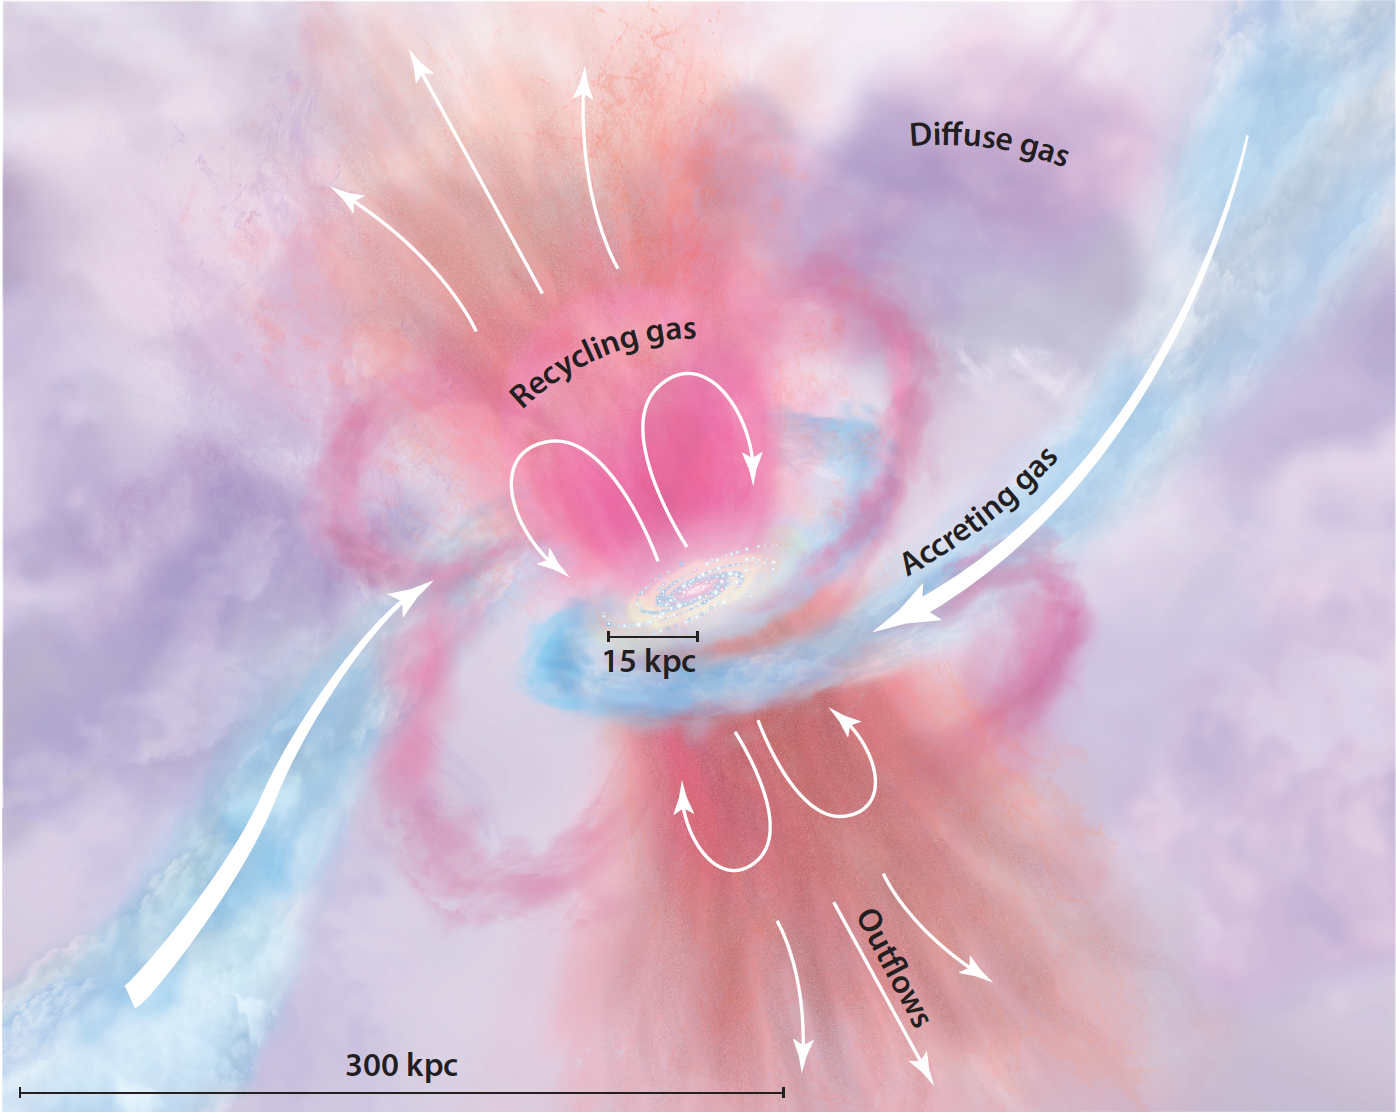
\includegraphics[width=0.8\textwidth]{plots_chp1/CGM_Tumlinson_2017.png}
 \caption[A general view of a galaxy's circumgalactic medium (CGM)]{An idealised illustration of the circumgalactic medium offered by \citet{tumlinson2017}.}
 \label{fig:CGM-Tumlinson2017}
\end{figure}

The processes and features referred to in Fig. \ref{fig:CGM-Tumlinson2017} are: (a) the inflow or accretion of pristine gas from the IGM; (b) outflows of gas that may be driven by either stellar and/or AGN feedback events; (c) infall of metal-rich gas that has been expelled from the galaxy at velocities $\varv < \varv_{esc}$ (below the escape velocity); (d) diffuse extensions of low surface-brightness gas. Provided that the cold molecular gas that fuels star-formation is affected by one of or a combination of these mechanisms, the flow of baryons - gas as well as metals or dust - into and out of the CGM plays a very significant role in the evolutionary path that a galaxy follows.

The concept of a CGM only emerged in the astronomy lexicon rather recently. During this time, both observations and simulations, which have improved over the years with the development of new instruments on telescopes and faster computing, have been invoked to study the CGM in greater detail. Observationally, some of the main methods for studying the CGM are: (a) detecting absorption lines in spectra in the transverse direction on the projected plane of a galaxy; (b) mapping out line-emission; (c) stacking spectra from faint sources; (d) detecting line emission and absorption ``down-the-barrel'' or along the line-of-sight; (e) simulating and modelling CGM processes using hydrodynamical simulations and semi-analytic models. Each of these methods have been succinctly outlined by \citet{tumlinson2017} as the following:

(a) The absorbing gas within the CGM of a galaxy, when viewed against a background quasar, is defined by several parameters. The first of these is column density which is simply the number of absorbing ions or atoms per unit area along a sight-line, Doppler widths given by the $b$ parameter which is defined as $b^2 = 2kT/m + b_{nth}$ in which $k$ is the Boltzmann constant, $T$ the temperature of the gas medium, and $m$ is the gas particle mass and $b_{nth}$ is due to intrinsic broadening of emission lines as a result of gas turbulence. Redshifts of the absorbing gas are obtained by fitting Voigt profiles to continuum-corrected absorption lines in nearby galaxies \citep[e.g.,][]{Lehner2015,Bowen2016}, distant lensed quasars \citep{RauchHaehnelt2011,Rubin2015} and distant radio galaxies \citep{vanojik1996,wilman2003}. 

(b) Additionally, emission line maps of radiation from CGM have been made with the use of deep narrow-band imaging \citep{Prescott2015,Arrigoni-Battaia2016}, integral field unit (IFU) spectrographs such as the Keck Cosmic Web Imager (KWCI) as seen in \citet{Cai2018} as well as on the Very Large Telescope (VLT) with Multi-unit Spectroscopic Explorer (MUSE) which provides a spectrum for every pixel in the instrument's field of view \citep[e.g.,][]{Cantalupo2014}. 

(c) Stacking spectra is gainful for detecting weak or faint absorption through the co-addition of hundreds to thousands of spectra from large surveys. (d) Emission and absorption are detected ``down-the-barrel" or along the line-of-sight using spectroscopy. This method relies on line and continuum emission to be by starlight and possibly also an AGN within a galaxy. The emission serves as a background source without which constraints on the absorbing gas in front of the emission line region would not be possible. This way of detecting CGM gas properties is commonly adopted when observers look for direct evidence of inflowing and outflowing gas by tracing where redshifted and blueshifted emission occurs along the line-of-sight \citep{Steidel2010,Heckman2015}. (e) Simulations of a galaxy CGM's temperature, metallicity, and density have been and continue to be an essential way of grappling the effects of baryon flows over cosmological time-scales as they offer a continuous or evolving view of the associated processes \citep{SomervilleDave2015}.

%phases of the CGM
Another important aspect of the CGM is that it is a multi-phase gas medium within which ionised, molecular and neutral gas complexes can be found. The phases of the CGM have been inferred from hydrodynamic simulations such as those of Fig. \ref{fig:phase-diagram-gas-Torrey2019} from \citet{Torrey2019}, which illustrates the expected baryon phases within the gravitationally bound gas halo at $z=0$ as a function of temperature and density. Hot, diffuse gas with $\log{(T/K)} \gtrsim 7$ is predicted by simulations as well and has also been observed in soft X-ray emission \citep{AndersonBregman2010}. The warm, ionised gas medium generally has temperature within the approximate range of $\log{(T/K)} \simeq 4.5 - 6$ with slightly cooler ionised gas having temperatures of $\log{(T/K)} \simeq 4.$ More information about the ionisation conditions and temperatures of ionised gas can be drawn from photoionisation equilibrium models (PIE) such as the spectral synthesis modelling code \pkg{cloudy} \citep{Ferland2013}. 

\begin{figure}
 \centering
 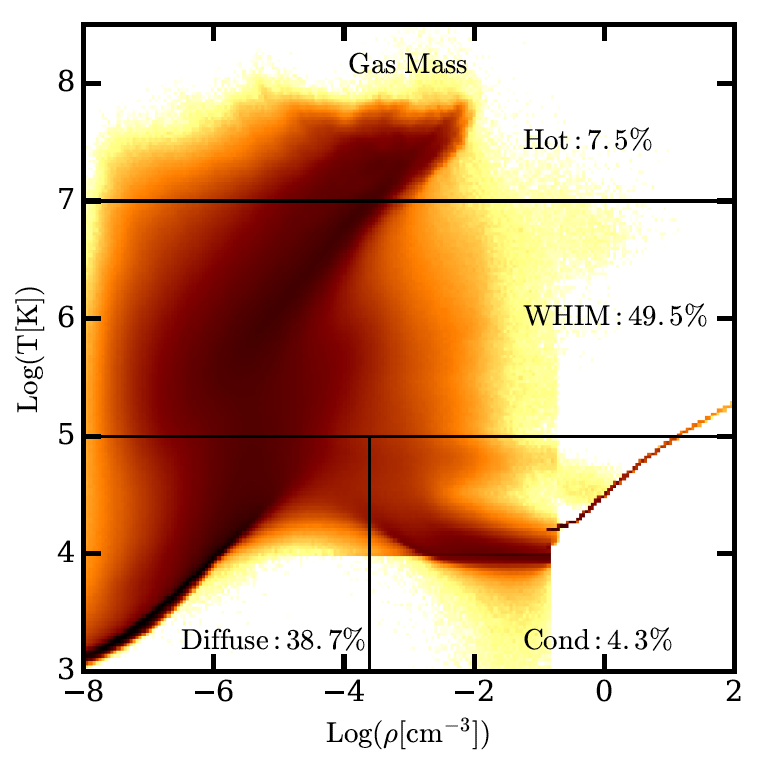
\includegraphics[width=0.7\columnwidth]{plots_chp1/Phase_diag_Torrey2019}
 \caption[Phase diagram of a simulated gas-mass distribution at $z=0$]{Phase diagram of gas-mass distribution at $z=0.$ The boundaries between the different gas phases are given along with the fraction of gas phase to the total gas budget. The gas phases are a hot ($\log{(T/K)} > 7$), warm-hot intergalactic medium (WHIM; $5 < \log{(T/K)} < 7$), diffuse ($\rho < 1000\rho_{\rm c}\Omega_{\rm c}$, $\log{(T/K)} < 5$) and condensed gas ($\rho > 1000\rho_{\rm c}\Omega_{\rm c}$, $\log{(T/K)} < 5$) masses which were coined by \citet{Dave2001} and \citet{Haider2016}. $\Omega_{\rm c}$ and $\rho_{\rm c}$ are critical densities.}
 \label{fig:phase-diagram-gas-Torrey2019}
\end{figure}

One of the major issues facing CGM studies, however, is that of the so-called ``missing baryons''. This has been evinced by CGM masses of low to high luminosity galaxies being lower than the expected cosmological baryon to mass density parameter ratio of $\Omega_{\rm b}/\Omega_{\rm M}=0.16$ determined from observations from the Planck Mission \citep{Planck2016}. Also, measurements of galaxy halo masses have proved that the total measured masses of baryons in galaxies are lower than that which is predicted by  $\Lambda$CDM (cold dark matter) cosmology. In other words, $M_b \ll (\Omega_{\rm b}/\Omega_{\rm M})M_h$ where $M_b$ is the total baryon mass, and $M_h$ the halo mass. An example of this is illustrated in Fig. \ref{fig:CGM-baryon-budget-Tumlinson2017} where the surface gas densities of multiple gas phases and dust when added do not account for the gas surface density predicted by $\Lambda$CDM cosmology. In general, many galaxies appear to be missing up to $80\%$ of their baryons meaning that the majority of baryons in the CGM are currently unaccounted for. It has been suggested that the missing baryons may be contained within the diffuse, hot halo gas medium. The validity of this will be tested in current as well as upcoming X-ray missions such as {\it eRosita} \citep{Merloni2012}, which was launched in July 2019, {\it NuSTAR} (Nuclear Spectroscopic Telescope Array) \citep{Harrison2013} and {\it ATHENA} \citep{Nandra2013}. 

\begin{figure}
 \centering
 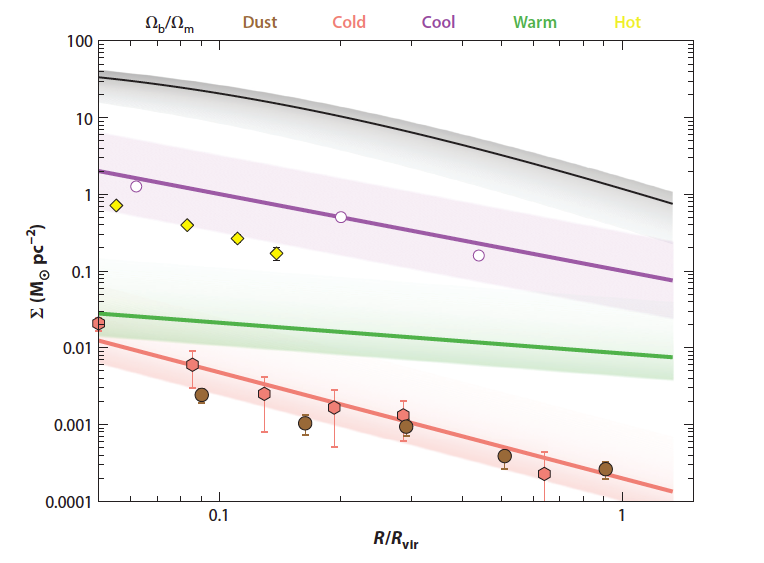
\includegraphics[width=0.8\textwidth]{plots_chp1/CGM_missing_baryons_Tumlinson_2017}
 \caption[Multi-phase CGM mass surface-density profiles]{Synthesis of CGM mass surface-density profiles of multi-phase components compared to the Navarro-Frenk-White (NFW) profile (black) prediction scaled by $\Omega_{\rm b}/\Omega_{\rm M}$ for a dark-matter mass of $M_{\rm DM}/\rm{M}_\odot = 2\times10^{12}.$ The density profiles are for cold gas (salmon) from \citet{ZhuMenard2013a}, cool gas (purple) from \citet{Werk2014}, warm gas (green) traced by \ion{O}{VI} ions \citep{Tumlinson2011,Peeples2014}, hot X-ray emitting gas (yellow) \citep{Anderson2016} and dust (brown) \citep{Menard2010}. }
 \label{fig:CGM-baryon-budget-Tumlinson2017}
\end{figure}

The CGMs of radio galaxies can be studied in great detail because of their bright, extended emission line regions which act as proverbial flash-lights, illuminating the foreground gas within the halo. Observing the CGM also permits one to look for evidence of kinetic feedback beyond just the ISM. 

\subsection{The CGMs of High-redshift Radio Galaxies } 
Observing the kinematics, morphology and ionisation state of gravitationally bound halo gas found around HzRGs is pivotal to understanding how the mechanical power of the radio jets play a role in moderating a galaxy's gas supply. Thankfully, evidence for jet-gas interactions within the gaseous haloes of radio galaxies is plentiful. One of the most effective ways to probe kinematically perturbed gas within the haloes of HzRGs is with emission-line-width measures, particularly the lines that trace the warm, ionised gaseous medium. Most HzRGs are surrounded by giant complexes of ionised gas traced primarily by Ly$\alpha$ emission nebulae \citep{mccarthy1990a,reuland2003}. The Ly$\alpha$ nebulae of HzRGs are known to extend out to to diameters of up to $d \lesssim 200$ kpc. 

%Warm, ionised gas medium
In the rest-frame UV spectral regime spanning $1200 - 1800~\text{\AA}$, the ionised gas medium engulfing a galaxy is probed by rest-UV lines, the most pervasive of which is the Ly$\alpha\lambda$1216. Some of the common lines detected from HzRGs are shown by the composite spectrum of \citet{McCarthy1993} which is a compilation of observed spectral lines in radio galaxy spectra at $0.1 < z < 3$ (see Fig. \ref{fig:comp_spec_RGs}). The emission lines trace the warm, ionised gas regions which have temperatures of approximately, $T_{\rm{e}} \sim 10^{4}-10^{5}$ K, and particle densities of $n_{\rm{e}} \sim 10^{0.5} - 10^{1.5} \rm cm^{-3}$ which are gleaned from emission line diagnostics \citep{OsterbrockFerland2006}. In low density gas regions, forbidden lines which have low transition probabilities are also detected. 
After \citet{reuland2003} used narrow-band imaging to demonstrate that a sample of HzRGs are engulfed by \lya~emitting haloes extending of sizes $d \simeq 100-200$ kpc, it became clear that giant \lya~nebulae are common to many HzRGs. 

\begin{figure}
\centering
  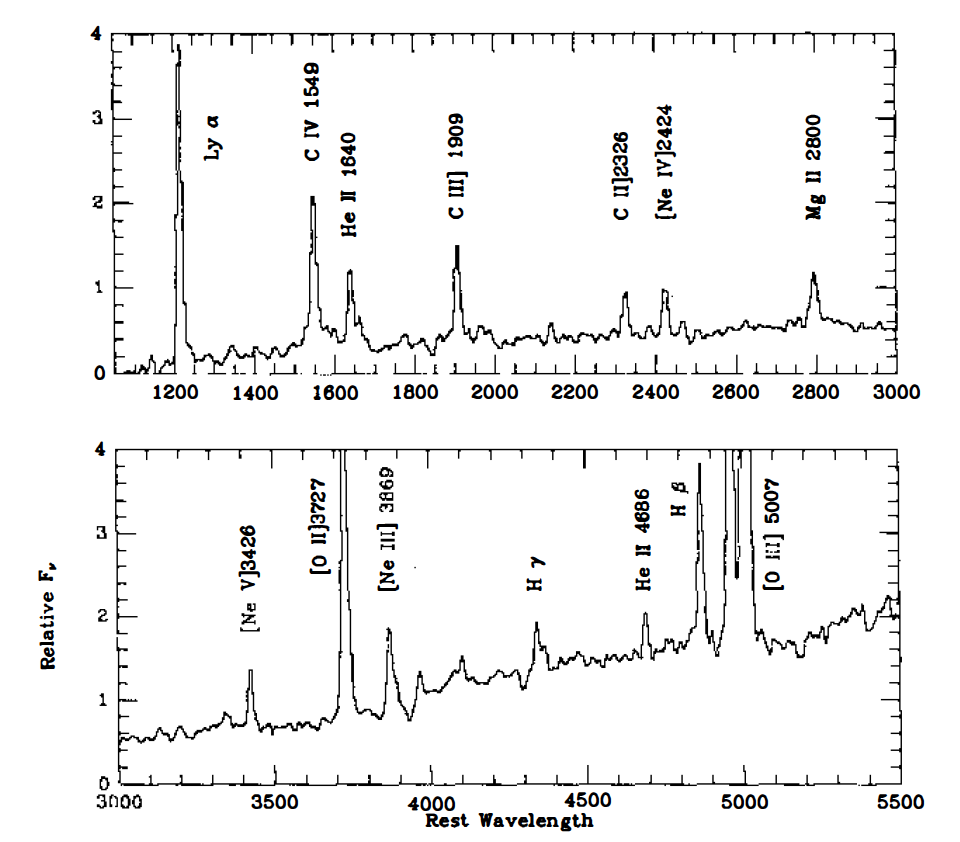
\includegraphics[width=0.65\textwidth]{plots_chp1/UV_spectrum_McCarthy2003}
  \caption[Composite radio galaxy spectrum from galaxies at $0.1 < z < 3$]{Composite radio galaxy spectrum obtained from galaxies at $0.1 < z < 3$ comprising data from the telescopes, Kitt Peak 4 m, Lick 3 m, and Palomar 5 m with $2.5'' \times 3"$ apertures from \citep{McCarthy1993} }
  \label{fig:comp_spec_RGs}
\end{figure}

The high surface-brightness regions within the extended haloes of HzRGs are characterised by turbulent kinematics traced by ionised gas line tracers that are broadened to line-widths of $\rm FWHM \gtrsim 1000$ km s$^{-1}.$ The emission-line gas traced can have luminosities well up to $\rm 10^{44}~erg~s^{-1}$ \citep{mccarthy1996,villar-martin1999a}. In addition to being highly energetic and consisting of turbulent gas motions, the inner halo regions of HzRGs also have clumpy morphologies observed with rest-UV/optical imaging from {\it HST} and spectroscopy from {\it Keck} \citep{humphrey2006,Villar-Martin2006}. The outskirts of HzRG haloes tend to have more quiescent kinematics with line-widths of approximately $\rm FWHM \simeq 100$ km s$^{-1}$ and smoother rest-UV/optical morphologies consistent with gas that is dynamically relaxed \citep{villar-martin2003} (see Fig. \ref{fig:kinematics-ionised-Villar_Martin2003}). 

\begin{figure}[!ht]
 \centering
 \subfloat[]{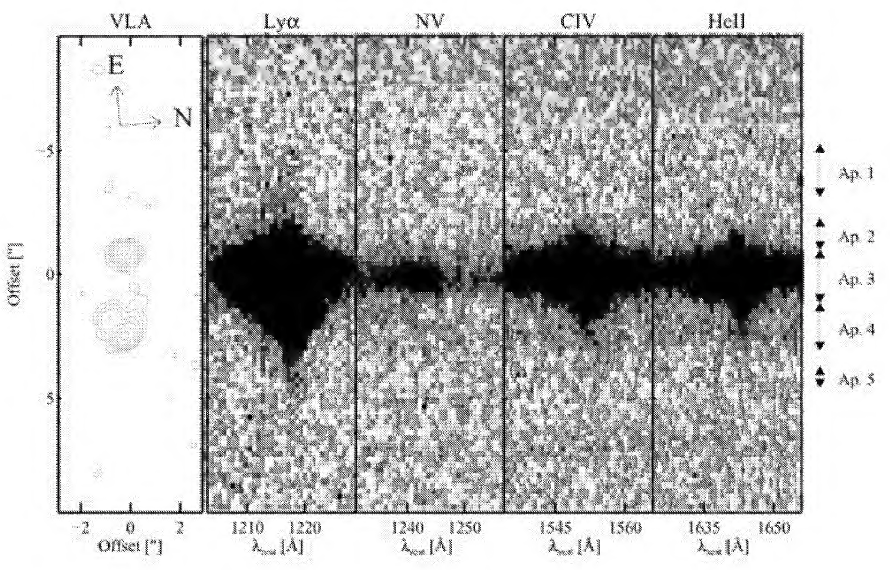
\includegraphics[width=0.7\textwidth]{plots_chp1/pos_velocity_Villar_Martin2003.png}}\\
 \subfloat[]{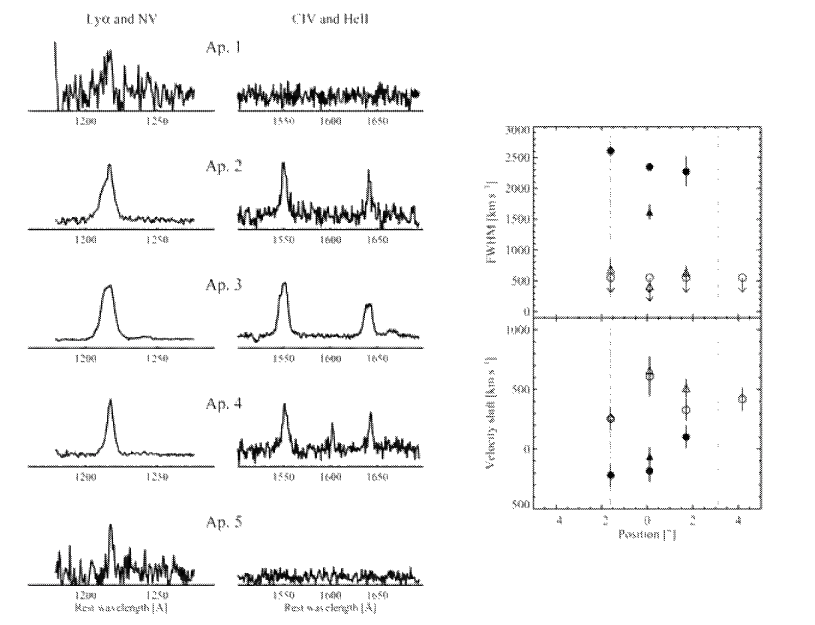
\includegraphics[width=0.7\textwidth]{plots_chp1/spectra_FWHM_vel_shift_Villar_Martin2003.png}}
     \caption[Keck 2D and 1D spectra from \citet{villar-martin2003}]{Panel (a): VLA radio map of the radio galaxy 1809+407 showing Keck 2D spectra (position-velocity diagrams) for Ly$\alpha$ $\lambda$1216, \ion{N}{v} $\lambda$1238, \ion{C}{iv} $\lambda$1550 and \ion{He}{ii} $\lambda1640.$ Panel (b): Spatially integrated spectra from the apertures labelled in panel a (left). The FWHM and velocity offsets relative to \ion{He}{ii} which marks the zero-velocity centroid. The symbols represented are circles for Ly$\alpha,$ and triangles for \ion{He}{ii}; filled symbols for broad components and non-filled symbols for narrow kinematic components of an emission line \citep{villar-martin2003}.} 
 \label{fig:kinematics-ionised-Villar_Martin2003}
\end{figure}

Recent observations of HzRGs using IFU spectroscopy have confirmed much of what has been known of the kinematics and morphology of their gaseous haloes. The IFU spectrograph MUSE, which has a sufficiently good sensitivity to probe extended diffuse emission in the optical, has been important in bringing about a spatially resolved view of emission from ionised gas in the extended gas haloes of distant radio galaxies. In \citet{swinbank2015}, narrow-band imaging of the $z=4.1$ radio galaxy (TN J1338-1942) reveals its colossal $\sim$150 kpc diameter Ly$\alpha$ nebula. Mapping out the velocity in this source showed that it has a velocity gradient of up to $\sim$1000 km s$^{-1}$ along the extent of its nebula (as shown in Fig. \ref{fig:TNJ1338-Swinbank2015}). MUSE IFU data was also important in showing the morphologies of emission in the galaxy MRC 0943-242 from Ly$\alpha$ as well as other rest-UV lines such as \ion{He}{ii} $\lambda1640$, \ion{C}{iv} $\lambda1550$ and \ion{C}{iii]} $\lambda1907$ and \ion{C}{ii]} $\lambda2326$ \citep{Gullberg2016a,Silva2018}. 

\begin{figure}[!ht]
 \centering
 \subfloat[]{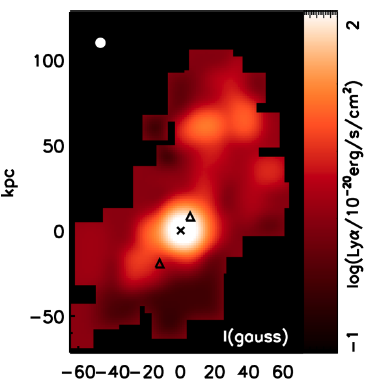
\includegraphics[width=0.5\columnwidth]{plots_chp1/Ly_alpha_intensity_Swinbank2015}}\\
 \subfloat[]{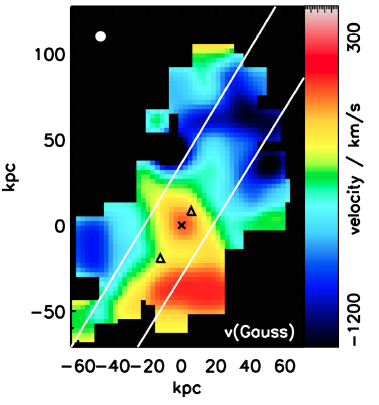
\includegraphics[width=0.5\columnwidth]{plots_chp1/vel_map_Swinbank2015}}
 \caption[Intensity and velocity map from \citet{swinbank2015}]{Panel (a): An intensity map of the underlying Ly$\alpha$ emission profile (modelled by a Gaussian). Panel (b): Velocity map of the Gaussian emission profile from panel (a). The nucleus is shown as a cross and the radio hotspots as triangles. The white lines represent the orientation of the slit along which the velocity shear and \ion{H}{i} column density profiles are seen in spectra extracted from a 9-h observation of the source using the VLT and integral field unit (IFU) spectrograph MUSE (Multi-unit Spectroscopic Explorer) \citep{swinbank2015}.}
 \label{fig:TNJ1338-Swinbank2015}
\end{figure}

The neutral phase of the gas haloes of HzRGs can be probed via Ly$\alpha$ absorption. The absorption troughs superimposed by Ly$\alpha$ emission lines originate from neutral hydrogen located in front of the extended emission line regions along the line-of-sight \citep{rottgering1995,vanojik1997}. The neutral gas which when fit with Voigt profiles is found to have neutral hydrogen (\ion{H}{i}) column densities of $ N_{\rm \ion{H}{i}} /\rm{cm}^{-2} \simeq 10^{18}-10^{20}$ may be associated with the galaxy (located within its ISM or CGM) or be a part of intervening absorption and therefore part of the Ly$\alpha$ forest with $N_{\rm \ion{H}{i}} /\rm{cm}^{-2} \simeq 10^{13} - 10^{15}$ \citep{wilman2004}. In addition to Ly$\alpha,$ other resonant lines such as \ion{C}{iv} $\lambda1550,$ \ion{N}{v} $\lambda1238$ and \ion{Si}{iv} $\lambda1402.$ The neutral phase can also be probed via direct \ion{H}{i} 21cm absorption which has already been done for the $z=3.4$ galaxy B2 0902+34 \citep{Uson1991}. With higher sensitivity radio interferometers which will come online within the next two decades, this direct detection of \ion{H}{i} will become possible for fainter sources. 

The molecular phase of HzRG haloes can be traced via the various fine-structure transitions of the carbon monoxide (CO) molecule. $^{12}$CO emission lines trace molecular hydrogen (H$_2$) due to collisional excitation of CO by the H$_2$ molecule which result in emission from the rotational transitions $J=1\rightarrow0, 2\rightarrow1, 3\rightarrow2, 4\rightarrow3$ and $5\rightarrow4$ \citep{SolomonvandenBout2005}. Several HzRGs have been detected in these CO transitions \citep{Scoville1997,Alloin2000,deBreuck2003,Papadopoulos2000,
Greve2004,deBreuck2005,Klamer2005,Ivison2008,Emonts2014,emonts2015,Gullberg2016b}. The observations that provided these results were obtained from milimetre/sub-milimetre interferometry on instruments such as Australia Telescope Compact Array (ATCA), Owens Valley Radio Observatory (OVRO), IRAM 30 m telescope, Plateau de Bure Interferometer (PdBI), Atacama Pathfinder Experiment (APEX) and the Atacama Large Millimeter/sub-millimeter Array (ALMA) among others. 

\citet{PapadopoulosGreve2004} were first to demonstrate that emission from the fine-structure transitions in atomic carbon can trace H$_2$ in low-redshift ($z\sim0.018 - 0.043$) ultra-luminous infrared galaxies (ULIRGs). The study showed that the scatter in the [\ion{C}{i}]/CO luminosity ratio is small; in other words, the H$_2$ masses derived from [\ion{C}{i}] and CO lines are consistent. Since then, [\ion{C}{i}]$^3$P$_1 - ^3$P$_0$ and [\ion{C}{i}]$^3$P$_2 - ^3$P$_1$ have been widely used to trace the molecular clouds from which stars form \citep{Alaghband-Zadeh2013,Bothwell2017,Popping2017,Andreani2018,Lelli2018,emonts2018,
Nesvadba2019,Man2019}. A remarkable example of [\ion{C}{i}](1-0) detections that extend far out into the CGM of the Spiderweb Galaxy is presented in \citet{emonts2018} (shown in Fig. \ref{fig:CI-Spiderweb-Emonts2018}). 

\begin{figure}
 \centering
 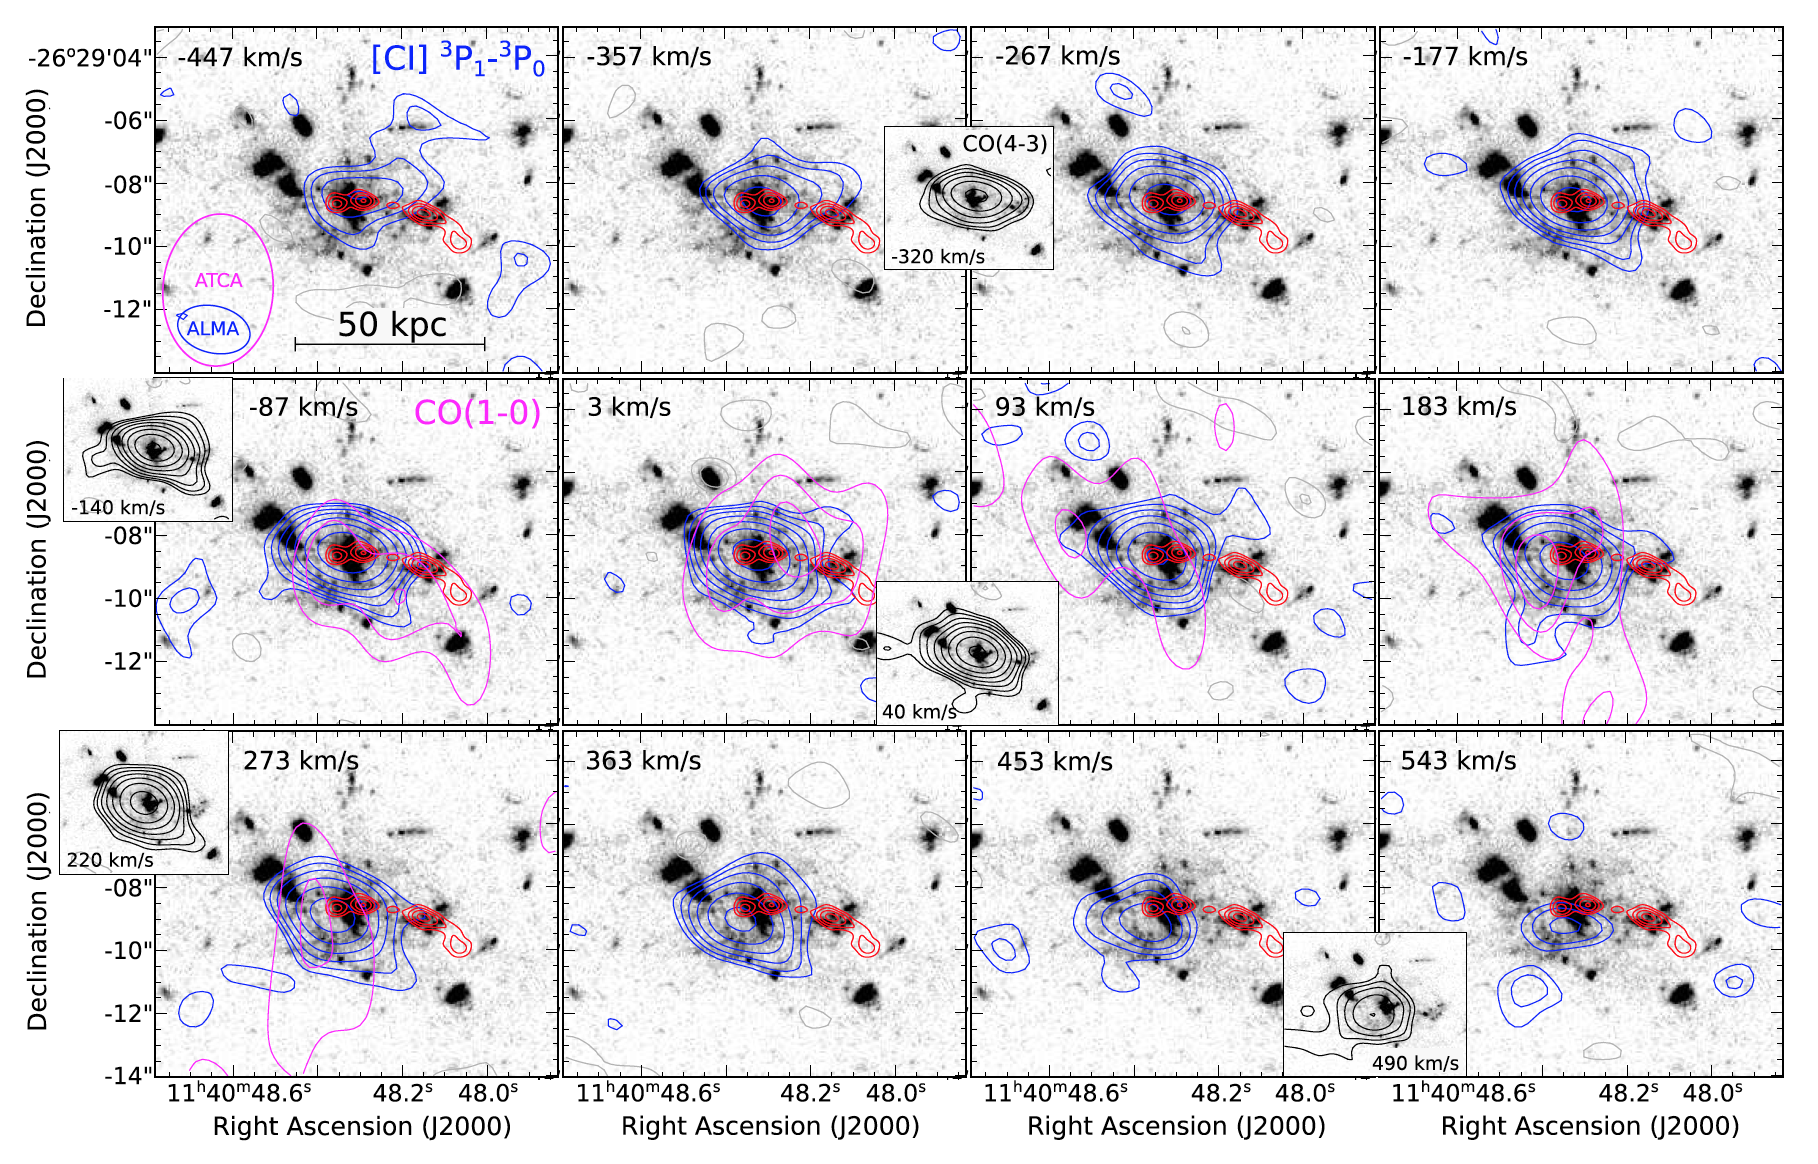
\includegraphics[width=\textwidth]{plots_chp1/Spiderweb_glx_CI_Emonts2018.png}
 \caption[Channels maps of CO(1-0) in MRC1138-262 from \citet{emonts2018}]{Channels maps of the [\ion{C}{i}]$^3$P$_1-^3$P$_0$ emission (blue contours) overplotted over an HST/ACS F475W+F814W image from \citet{Miley2006}. The magenta contours indicate the previously detected CO(1-0) emission and the insets show prominent features detected at other velocity channels. Contour levels of [\ion{C}{i}] and CO(4-3) start at $2\sigma$ and increase by a factor of 1.5, with $\rm \sigma=0.07~mJy~beam^{-1}$ (negative contours are shown in grey). CO(1-0) contour levels are at $2\sigma,$ $3\sigma,$ $4\sigma,$ $5\sigma$ for $\rm \sigma=0.086~mJy~beam^{-1}.$ The red contours indicate the 36 GHz radio continuum from \citet{Emonts2016}.}
 \label{fig:CI-Spiderweb-Emonts2018}
\end{figure}

Overall, observations of distant radio galaxies obtained in the optical, infrared, mm/sub-mm have provided a substantial proportion of evidence suggesting that the gaseous nebulae around HzRGs can be extensive in size $d \gtrsim 200$ kpc. Thermal broadening of line such as Ly$\alpha$ which trace the ionised gas in the halo have suggested that the innermost regions of galaxy haloes up to $d \lesssim 50$ kpc from the AGN more turbulent kinematics than the regions of ionised gas further out \citep{villar-martin2003}. This is quite indicative of how influential radio jets may be in driving ISM gas kinematics. 

Still some questions remain. Do the radio jets alone drive these extreme kinematics? The neutral gas traced by absorption in the resonant line Ly$\alpha$ reveals what may be absorption from the Ly$\alpha$ forest or neutral reservoirs of gas within the CGMs of HzRGs. How does this neutral gas find its way into the CGM - is it accreted along filaments from the IGM or expelled from the host galaxy by AGN feedback? If so how may we observe this? As mentioned earlier, molecular hydrogen is traced by CO and [\ion{C}{i}] lines show that giant molecular clouds also occur up to hundreds of kpc from their host galaxy nuclei within the CGM. Does this H$_2$ gas have primordial origins or is it detected within the CGM as a result being expelled by an AGN feedback event? 

In order to answer questions concerning the kinematics, chemical and morphological structure of the CGMs of distant radio galaxies, deeper observations of such galaxies are required. The CGM maintains the imprints of baryon flows which makes it a kind of forensic tracer for the astrophysical processes that are central to how a galaxy evolves. Coupling these observations with the results of resolved simulations matched in distance scale will provide better insight into the workings of gas within CGM.

% -------------------------------------------------------------------------------------
%           												Section 1.4
% -------------------------------------------------------------------------------------
\section{General Thesis Outline}
% What is the purpose of this thesis?
% What does it aim to achieve ?
% How does it do this?

The main goal of this thesis is to demonstrate that the mechanical power of radio jets play a significant role in altering the morphology, kinematics and ionisation state of the multi-phase gaseous environment from the ISM to the CGM at the $\gtrsim$200 kpc distance scale. We explore this topic in three separate studies. 

\subsection{Chapter 2}
In chapter 2, I have explored the influence of radio-jets on the $<1$Mpc-scale environment density. With the use of a nearest neighbour pseudo-3D density measure, I quantify group scale environments of 2716 radio sources within a 100 deg$^2$ area of the Stripe 82 equatorial field. The radio-jet power is traced using 1.4 GHz luminosities (L$_{1.4~\rm GHz}$) detected from the VLA in the CnB configuration. A statistical correlation test between the galaxy number densities measured to the 2$^{nd}$ and 5$^{th}$ nearest neighbours and radio jet power for radio sources up to $z \sim 0.8$ is carried out. This is achieved by comparing the environment density measures of radio-selected AGN to optical sources that are matched by $K-$band magnitudes and $(g-K)$ colour indices. 

This chapter is based on a published paper of which I am the first author. Thus, I carried out the majority of the work which included scripting the \pkg{python} code required to obtain all of the main results. I was also responsible for assembling the initial and follow-up drafts of the publication which included finding most of the relevant literature required to interpret and discuss our findings. 

\subsection{Chapter 3}
Chapter 3 is a single-source paper. In it, I have used MUSE data to explore the kinematics of ionised and neutral gas within the ISM and CGM of a $z=2.92$ radio galaxy, MRC 0943-242. I did so by parametrising rest-UV lines detected around the nucleus in terms of their emission components which I fit using multivariate Gaussian functions. The resonant rest-UV lines permit us to quantify absorption and I fit these with composite Voigt and Gaussian functions. I compared the column densities obtained from Voigt profile fitting to predictions based on photoionisation models with \pkg{cloudy}. The dominant ionising mechanism powering the metal-rich absorbers is also determined in addition to the distances of the absorbers from the ionising source. 

For this published paper, I reduced the data via the standard ESO reduction pipeline, \pkg{esorex}, for IFU data which produced the final datacube which was analysed to obtain the results reported via \pkg{python} scripts that I wrote. As the first author, I drafted and completed the final draft for submission to the journal. 

\subsection{Chapter 4}
In chapter 4, I have taken ALMA [\ion{C}{i}]$^3$P$_1$ - $^3$P$_0$ line and continuum observations within a $40 \times 40$ arcec$^2$ field of view for seven radio galaxies between $2.9 \lesssim z \lesssim 4.6.$ The [\ion{C}{i}](1-0) line traces molecular hydrogen, which I have used to constrain the masses and kinematics of H$_2$ masses in the ISM and CGM gas regions of the HzRGs. 

For this chapter, I reduced and imaged the interferometric observations using the  reduction pipeline, \pkg{casa} (Common Astronomy Software Applications). I developed the \pkg{python} code required to obtain the results shown in the form of images and spectra and assembled the literature needed for the interpretation and discussion. 